\documentclass[11pt,a4paper]{article}
\usepackage[utf8]{inputenc}
\usepackage[T1]{fontenc}
\usepackage[brazilian]{babel}
\usepackage{geometry}
\geometry{margin=2.3cm}
\usepackage{graphicx}
\usepackage{booktabs}
\usepackage{longtable}
\usepackage{array}
\usepackage{float}
\usepackage{xcolor}
\usepackage{amsmath}
\usepackage{enumitem}
\usepackage{caption}
\usepackage{hyperref}
\hypersetup{colorlinks=true, linkcolor=blue!50!black, urlcolor=blue!50!black}
\captionsetup{font=small, labelfont=bf}
\setlist{itemsep=2pt, topsep=4pt}
\graphicspath{{figs/}}
\newcommand{\tg}[1]{\texttt{\detokenize{#1}}}

\title{OCSVM e CNN-1D por grupo de sinal:\\ treino único, retreino mensal e o limite dos dados atuais\\
\large Turbina TC-33003A -- Cabiúnas}
\author{Equipe de Modelagem}
\date{18 de outubro de 2026}

\begin{document}
\maketitle

\begin{abstract}
Este relatório compara duas famílias de modelo na mesma arquitetura de produção: um modelo por grupo de sinal
(temperatura, vibração e pressão de óleo), mais um canal de alarmes de processo e uma camada de decisão por regras.
A primeira família é a OCSVM de produção, com treino único. A segunda é um autoencoder convolucional 1D (CNN-1D AE),
com retreino mensal desde 01/2025. O relatório descreve como os canais foram separados, como cada modelo foi treinado
e em que período, e mostra a série temporal dos dois lado a lado: sinal original, pontos anômalos, trips previstos e
episódios que não são trip. O CNN-1D mensal pega os 8 trips com antecedência, inclusive os 5 de 2025 que ele não viu
no treino. Mas gera 25\% mais falsos positivos (45 contra 36 desde 01/2025), e somá-lo à OCSVM como canal extra corta
só 6\% (9\% fora da amostra). O diagnóstico dos 62 episódios da produção mostra por quê. Quase todo episódio, acerto ou erro, nasce do
mesmo par de alarmes recorrentes de processo (\tg{PI_6240319_AL} e \tg{PAL_6240315}) mais um modelo aceso, quase
sempre a vibração. Trips e falsos positivos têm a mesma composição, e regras sobre alarmes e votos não conseguem
separá-los com os dados atuais. O relatório termina com os problemas desses dados e com o que é preciso obter para
avançar.
\end{abstract}

\tableofcontents
\newpage

%=====================================================================
\section{Contexto e pergunta}
%=====================================================================

A pipeline vigente detecta precursores de trip da turbina TC-33003A com \textbf{três modelos isolados, um por grupo
de sinal}, e um \textbf{quarto canal sem modelo}, aceso por 24~h depois de cada alarme de cinco tags de processo. As
saídas binárias dos quatro canais entram numa camada de decisão de regras fixas: voto $\geq 2$, filtro de 45~min e
refratário de 48~h. Com OCSVM nos três grupos, ela detecta os 8 trips do histórico com 2,88 falsos positivos (FP)
por mês de operação.

A frente de \emph{disputa entre modelos} (D1) manteve a camada de decisão congelada e perguntou se outra família de
modelo, no lugar da OCSVM em cada grupo, mantém os 8 trips com pelo menos 25\% menos FP. Foram testados isolation
forest, autoencoder denso, PCA ($T^2$/$Q$) e CNN-1D AE, com treino único e com retreino mensal. Nenhuma combinação
passou no critério. Este relatório se concentra nas duas famílias que mais interessam à operação:

\begin{itemize}
  \item \textbf{OCSVM}: o modelo de produção, com treino único (e o teste de retreino mensal, C1);
  \item \textbf{CNN-1D AE}: o único candidato que, com retreino mensal, pegou os 8 trips também fora da amostra de
        treino, e o único que antecipou um trip recente bem mais cedo que a OCSVM (09/12/2025: 21,1~h contra 8,4~h).
\end{itemize}

Depois do placar, o relatório investiga \emph{de onde vêm} os pontos anômalos que não são trip, e se dá para
eliminá-los com regras depois do treino sem perder os trips. A resposta leva a uma conclusão sobre os dados
disponíveis hoje (Seções~\ref{sec:diagnostico} a~\ref{sec:mais-dados}).

%=====================================================================
\section{Dados e períodos}
\label{sec:dados}
%=====================================================================

\begin{itemize}
  \item \textbf{Sinais:} \tg{sensores_full_2024_2026_30s.csv} (Dataset ClearML \tg{a97ba56b}), amostragem de 30~s,
        de 01/07/2024 a 20/04/2026 (1.895.041 instantes). A máquina está em operação (\tg{on}) 67,3\% do tempo no
        período inteiro e 75,8\% desde 01/2025. O resto são paradas longas, curtas e transientes.
  \item \textbf{Alarmes de processo:} \tg{alarmes_selecionados_turbina_a.csv}, mesmo Dataset. São 3.757 ativações
        (\tg{ACT}) de 47 tags, de 01/2022 a 18/04/2026, das quais 1.914 desde 07/2024.
  \item \textbf{Trips:} 8 eventos curados (\tg{FALHA_CURADA}), numerados T1 a T8 em todo o relatório
        (Tabela~\ref{tab:trips}).
  \item \textbf{Corte fora da amostra:} 01/07/2025 (\tg{AUTOML_OOS_SPLIT_DATE}). Antes dele estão 5 trips; depois, 3.
\end{itemize}

\begin{table}[H]
\centering\small
\caption{Os 8 trips do período. ``Dentro'' e ``fora'' referem-se ao corte de 01/07/2025.}
\label{tab:trips}
\begin{tabular}{llll}
\toprule
& data e hora & amostra (corte 01/07/2025) & visto no treino do CNN-1D mensal (1d)? \\
\midrule
T1 & 27/02/2025 08:38 & dentro & não \\
T2 & 17/03/2025 18:16 & dentro & não \\
T3 & 07/04/2025 21:18 & dentro & não \\
T4 & 11/04/2025 17:02 & dentro & não \\
T5 & 29/04/2025 03:04 & dentro & não \\
T6 & 04/11/2025 06:22 & fora & não \\
T7 & 09/12/2025 08:36 & fora & não \\
T8 & 26/02/2026 15:34 & fora & não \\
\bottomrule
\end{tabular}
\end{table}

\subsection{Períodos de treino de cada experimento}

A Figura~\ref{fig:periodos} resume os períodos.

\begin{itemize}
  \item \textbf{OCSVM de produção (treino único):} o modelo de cada grupo é treinado uma vez, com uma subamostra de
        50.000 pontos do \emph{normal} entre 01/07/2024 e 30/06/2025. O normal exclui 24~h em volta de cada alarme e
        os buracos longos. Depois, o modelo pontua o período inteiro. Os 5 trips de 2025 estão dentro do período de
        treino (como parte do normal, fora da janela de alarme).
  \item \textbf{OCSVM mensal (teste C1):} retreino no início de cada mês desde 07/2025, com todo o normal anterior
        (janela expansiva). Só pontua depois de 07/2025.
  \item \textbf{CNN-1D mensal, rodada 1c:} igual ao C1, com CNN-1D no lugar da OCSVM. Só pontua depois de 07/2025.
  \item \textbf{CNN-1D mensal, rodada 1d:} retreino mensal desde \textbf{01/01/2025} (16 retreinos). O primeiro modelo
        usa o normal de 07 a 12/2024, e cada mês é pontuado pelo modelo treinado até a véspera. Assim os 5 trips de
        2025 caem \emph{fora} do treino deste braço, e os 8 trips ficam julgáveis.
  \item \textbf{Escolha do limiar (AutoML):} em todos os braços, o percentil do limiar e o debounce de cada grupo são
        escolhidos pela detecção dos alarmes do grupo \emph{depois} de 01/07/2025.
\end{itemize}

Por isso, a comparação OCSVM $\times$ CNN-1D mensal deste relatório usa o \textbf{recorte de 01/01/2025 a
20/04/2026}, em que os dois emitem flag. O recorte tem 11,8 meses de operação vigiada, dos quais 8,0 depois do
corte. Os números da OCSVM no período inteiro (2,885 FP/mês) aparecem só como referência.

\begin{figure}[H]
\centering
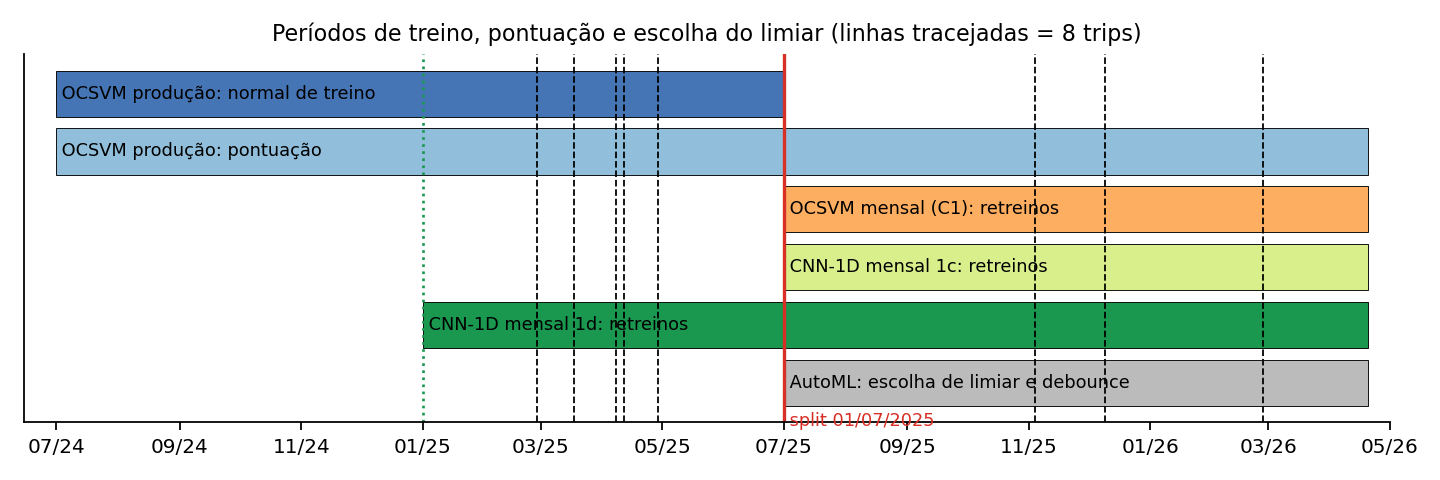
\includegraphics[width=\textwidth]{periodos.png}
\caption{Períodos de treino, pontuação e escolha do limiar de cada experimento. Linhas tracejadas: os 8 trips.
Vermelho: corte fora da amostra (01/07/2025). Pontilhado verde: início do retreino mensal da rodada 1d.}
\label{fig:periodos}
\end{figure}

%=====================================================================
\section{Como os canais foram separados}
\label{sec:canais}
%=====================================================================

A arquitetura usa \textbf{um modelo por mecanismo físico}, e não um modelo único com todos os sinais. O modelo único
foi testado antes e saturou em 6/8 trips (EXP35/36). Cada grupo é uma task separada no ClearML, com o mesmo código e
a mesma configuração de pré-processamento, e muda só a lista de sensores (Tabela~\ref{tab:grupos}).

\begin{table}[H]
\centering\small
\caption{Grupos de sinal. Configs de produção em \tg{configs/calibracao_v4_eq/}. Os ``alarmes de avaliação'' são
os que o AutoML usa para escolher limiar e debounce (só depois de 01/07/2025).}
\label{tab:grupos}
\begin{tabular}{p{2.6cm}p{4.2cm}p{3.0cm}p{4.2cm}}
\toprule
canal (config) & sensores do modelo & alarmes de avaliação & portões \\
\midrule
1 -- temperatura (EXP33) & \tg{TC382_03_A}, \tg{T5_AVG_A} & \tg{TC382_03_A}, \tg{T5_AVG_A} (40 alarmes) &
  carga, degrau (\tg{T5_AVG_A}), sensor congelado \\
2 -- vibração (EXP34) & 10 sensores \tg{TV_351X/Y_A} a \tg{TV_355X/Y_A} & \tg{TC382_03_A}, \tg{T5_AVG_A}
  (40 alarmes) & carga, degrau, sensor congelado \\
3 -- óleo (EXP38) & \tg{PI_0308}, \tg{PDIT_0305} & \tg{PALL_6240309} (\textbf{2 alarmes}) & sensor congelado \\
4 -- alarme de processo & sem modelo & -- & aceso por 24~h depois de cada ativação de \tg{PI_6240319_AL},
  \tg{PAL_6240315}, \tg{PDAL_6240302}, \tg{TC382_05_A} ou \tg{PAH_6240319} \\
\bottomrule
\end{tabular}
\end{table}

\paragraph{Pré-processamento (igual nos três grupos e nas duas famílias).}
\begin{itemize}
  \item \textbf{Features por sensor:} valor, delta de 1 passo, e mediana, desvio e tendência móveis em 4 janelas
        (12, 120, 480 e 2.880 pontos, ou seja, 6~min, 1~h, 4~h e 24~h), mais curtose, assimetria e fator de crista
        nas janelas de 120 pontos ou mais.
  \item \textbf{Normal de treino:} exclui 24~h em volta de cada alarme e os buracos longos. Outliers são clipados nos
        quantis 0,1\% e 99,9\%, e o z-score usa estatísticas só do treino.
  \item \textbf{Pós-modelo:} máscara operacional (só pontua com a máquina em operação) e portões de produção (carga,
        degrau, sensor congelado). Cada grupo gera o arquivo \tg{point_anomalies_all.csv}, com uma flag binária por
        instante de 30~s.
\end{itemize}

%=====================================================================
\section{Modelos e treinamento}
\label{sec:modelos}
%=====================================================================

\subsection{OCSVM}

One-Class SVM com kernel RBF ($\nu = 0{,}05$, $\gamma = $ \tg{scale}), treinada com 50.000 amostras do normal
(semente 42). O score de anomalia é a distância à fronteira com sinal invertido (\tg{-decision_function}). O AutoML escolhe o percentil do score no normal que
vira limiar e o \emph{debounce}, que é o número de pontos seguidos acima do limiar para acender
(Tabela~\ref{tab:hiper}).

\subsection{CNN-1D AE}

Autoencoder convolucional 1D (\tg{build_cnn1d_autoencoder} em \tg{src/cnn1d_ae/model.py}):

\begin{center}\small
entrada (60 passos $\times$ $n$ features) $\to$ Conv1D($f_1$, $k_1$, $s_1$) $\to$ Dropout $\to$ Conv1D($f_2$, $k_2$, $s_2$)
$\to$ Conv1DTranspose($f_2$, $k_2$, $s_2$) $\to$ Dropout $\to$ Conv1DTranspose($f_1$, $k_1$, $s_1$) $\to$
Conv1DTranspose($n$, 3); perda MSE, Adam.
\end{center}

\begin{itemize}
  \item \textbf{Janela:} 60 pontos (30~min). As janelas nunca cruzam buracos da série e, no treino, andam de 5 em 5
        pontos.
  \item \textbf{Score causal:} o erro de cada instante é o MSE da janela de 30~min que \emph{termina} nele, então o
        modelo não olha o futuro.
  \item \textbf{Busca de hiperparâmetros:} keras-tuner, RandomSearch com 10 tentativas. O espaço cobre filtros
        \{8, 16, 32, 64\}, kernels \{3, 5, 7, 9\}, strides \{1, 2\}, dropout de 0 a 0,4 e lr de $10^{-4}$ a
        $3\cdot10^{-3}$. Cada tentativa treina 20 épocas, com batch 1024 e early stopping de paciência 6.
  \item \textbf{Limiar:} escolhido pelo AutoML da mesma forma que na OCSVM.
\end{itemize}

\begin{table}[H]
\centering\small
\caption{Hiperparâmetros escolhidos pelo AutoML (semente 42). No CNN-1D mensal são os do último dos 16 retreinos;
nos três grupos a arquitetura vencedora foi a mesma: filtros 16/16, kernels 3/7, strides 2/2, dropout 0, lr
$3\cdot10^{-3}$.}
\label{tab:hiper}
\begin{tabular}{lllll}
\toprule
grupo & OCSVM: percentil / debounce & CNN-1D mensal: percentil / debounce & CNN-1D: janelas de treino \\
\midrule
temperatura & 97,5 / 1 & 95,0 / 1 & 195.269 \\
vibração & 95,0 / 4 & 95,0 / 12 & 196.953 \\
óleo & 99,9 / 12 & 99,9 / 12 & 244.680 \\
\bottomrule
\end{tabular}
\end{table}

\subsection{Treino único $\times$ retreino mensal}

No retreino mensal (\tg{_walkforward_fit_periods}, frequência \tg{MS}), cada mês refaz tudo do zero: normalização,
busca do tuner, modelo e limiar. O treino usa todo o normal anterior ao mês, e o mês é pontuado pelo modelo treinado
até a véspera. A ideia é acompanhar a deriva lenta dos sensores.

\begin{itemize}
  \item \textbf{Custo:} a OCSVM treina em minutos por grupo. O CNN-1D mensal da rodada 1d levou 1h10 (temperatura),
        2h50 (vibração) e 3h45 (óleo, rodando em paralelo) no Cica.
  \item \textbf{Memória:} o TF/Keras não devolve a memória de cada \tg{fit}, e a vibração estourou o worker no 8º
        mês. Correção: cada mês treina num processo filho (\tg{spawn}). O resultado ficou igual dentro do ruído
        do TF (diferença de $6\cdot10^{-5}$).
  \item \textbf{Execução em paralelo:} os 4 workers do Cica são a mesma máquina e a mesma GPU. A primeira vibração
        da 1d rodou junto com o óleo e morreu no 16º mês sem gerar resultado, embora marcada como \tg{completed}.
        Foi reenviada sozinha.
\end{itemize}

%=====================================================================
\section{Camada de decisão (regras) e régua (avaliação)}
\label{sec:regras}
%=====================================================================

São duas coisas diferentes, e as duas ficaram \textbf{congeladas} em todos os experimentos deste relatório.

\paragraph{Regras: o que geraria o alerta em produção.}
\begin{enumerate}
  \item Quatro canais binários: os 3 modelos e o canal 4.
  \item \textbf{Voto $\geq 2$:} pelo menos dois canais acesos ao mesmo tempo.
  \item \textbf{Filtro de 45~min:} o voto precisa durar 45~min seguidos.
  \item \textbf{Refratário de 48~h:} depois de um alerta, nada novo por 48~h.
\end{enumerate}

\paragraph{Régua: só avaliação, depois do fato.} Os alertas são agrupados em episódios (intervalos de até 2~h se
juntam). Cada episódio recebe uma classe:
\begin{itemize}
  \item \textbf{detecção}, se começa nas 48~h antes de um trip;
  \item \textbf{inconclusivo}, se não é detecção, mas a máquina para por 2~h ou mais até 48~h depois do fim
        (pode ser evento físico sem rótulo; não conta a favor nem contra);
  \item \textbf{falso positivo (FP)}, nos demais casos.
\end{itemize}
A antecedência é a distância entre o início da detecção e o trip. O custo é medido em FP por mês de operação.

\paragraph{Critério de aprovação (pré-registrado).} Manter 8/8 trips no recorte e 3/3 fora da amostra, com FP/mês
$\leq 75\%$ da OCSVM nos dois recortes: $\leq 2{,}288$ desde 01/2025 e $\leq 2{,}158$ depois de 07/2025.

%=====================================================================
\section{Resultados dos treinamentos mensais}
\label{sec:resultados}
%=====================================================================

\subsection{OCSVM com retreino mensal (C1)}

O retreino mensal da OCSVM foi testado antes do CNN-1D, com percentil e debounce fixos nos de produção
(Tabela~\ref{tab:c1}).

\begin{table}[H]
\centering\small
\caption{C1 -- OCSVM treino único $\times$ retreino mensal, fora da amostra (depois de 07/2025). Duty = fração do
tempo com o canal aceso.}
\label{tab:c1}
\begin{tabular}{lllll}
\toprule
braço & trips fora & antecedência (h) & FP fora (FP/mês) & duty temp $\cdot$ vib $\cdot$ óleo \\
\midrule
treino único (produção) & 3/3 & 13,7 $\cdot$ 8,4 $\cdot$ 3,8 & 23 (2,877) & 0,021 $\cdot$ 0,140 $\cdot$ 0,004 \\
retreino mensal & \textbf{2/3} & 13,7 $\cdot$ 8,4 $\cdot$ -- & \textbf{26} (3,252) & 0,024 $\cdot$ \textbf{0,072} $\cdot$ 0,003 \\
\bottomrule
\end{tabular}
\end{table}

O retreino mensal corta à metade o tempo aceso da vibração. Com isso some a coincidência que pegava o T8, e o FP
sobe em vez de cair. \textbf{Reprovado}: para a OCSVM, o retreino mensal é um risco, não uma alavanca de FP.

\subsection{CNN-1D: treino único e mensal desde 07/2025 (rodadas 1b e 1c)}

\begin{table}[H]
\centering\small
\caption{CNN-1D no lugar da OCSVM (canal 4 e regras iguais). ``Só X'' = CNN-1D só no grupo X, OCSVM nos outros.
$^*$Mensal desde 07/2025: só vale o recorte fora da amostra.}
\label{tab:1bc}
\begin{tabular}{lllll}
\toprule
combinação & trips (inteiro) & FP/mês inteiro & trips fora & FP fora (FP/mês) \\
\midrule
OCSVM (produção) & 8/8 & 2,885 & 3/3 & 23 (2,877) \\
CNN-1D treino único, 3 grupos & 6/8 & 3,503 & 2/3 & 28 (3,502) \\
CNN-1D treino único, só vib & 8/8 & 3,366 & 3/3 & 27 (3,377) \\
CNN-1D mensal$^*$, 3 grupos & -- & -- & 3/3 & 26 (3,252) \\
CNN-1D mensal$^*$, só vib & -- & -- & 3/3 & 24 (3,002) \\
\bottomrule
\end{tabular}
\end{table}

Com treino único, o CNN-1D perde trips. Com retreino mensal, pega os 3 trips fora da amostra e antecipa o T7 em
21,1~h, contra 8,4~h da OCSVM. Faltava saber se ele pegaria também os 5 trips de 2025. Essa é a rodada 1d.

\subsection{CNN-1D mensal desde 01/2025 (rodada 1d): os 8 trips}
\label{sec:1d}

\begin{table}[H]
\centering\small
\caption{Rodada 1d, recorte de 01/01/2025 a 20/04/2026 (11,8 meses de operação) e fora da amostra (8,0 meses).
Corte: 8/8 e $\leq 2{,}288$ FP/mês; 3/3 e $\leq 2{,}158$ fora.}
\label{tab:1d}
\begin{tabular}{llllll}
\toprule
combinação & trips & FP & FP/mês & trips fora & FP fora (FP/mês) \\
\midrule
OCSVM (produção) & 8/8 & 36 & 3,051 & 3/3 & 23 (2,877) \\
CNN-1D mensal, 3 grupos & 8/8 & 45 & 3,814 & 3/3 & 26 (3,252) \\
CNN-1D mensal só na vib & 8/8 & 42 & 3,560 & 3/3 & 24 (3,002) \\
CNN-1D mensal só no óleo & 8/8 & 36 & 3,051 & 3/3 & 23 (2,877) \\
CNN-1D mensal só na temp & \textbf{7/8} & 44 & 3,729 & 3/3 & 27 (3,377) \\
\bottomrule
\end{tabular}
\end{table}

\begin{figure}[H]
\centering
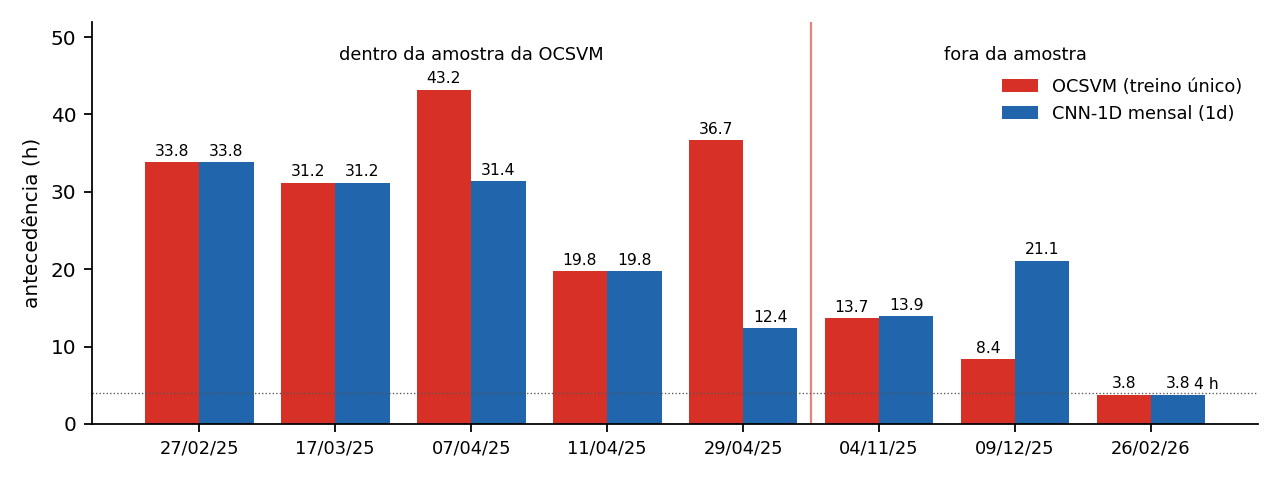
\includegraphics[width=0.9\textwidth]{antecedencia.png}
\caption{Antecedência por trip (h), OCSVM $\times$ CNN-1D mensal nos 3 grupos. Linha pontilhada: 4~h, a antecedência
mínima útil para a operação.}
\label{fig:antecedencia}
\end{figure}

\begin{itemize}
  \item \textbf{Detecção:} o CNN-1D mensal pega os 8 trips, inclusive os 5 de 2025, que ele não viu no treino. A
        OCSVM viu esses 5 dentro do período de treino, então o empate favorece o CNN-1D na generalização.
  \item \textbf{Antecedência:} o CNN-1D ganha no T7 (8,4 $\to$ 21,1~h, pela vibração) e perde no T3
        (43,2 $\to$ 31,4~h) e no T5 (36,7 $\to$ 12,4~h). Somando os 8 trips, são 167~h contra 191~h da OCSVM.
  \item \textbf{FP:} 45 contra 36 (+25\%), quando o critério pedia 25\% \emph{a menos}. A
        Figura~\ref{fig:fpmensal} mostra que o excesso se espalha pelo período, sem se concentrar num mês.
  \item \textbf{Veredito:} nenhuma combinação passa. O CNN-1D mensal empata em detecção e perde em FP.
\end{itemize}

\begin{figure}[H]
\centering
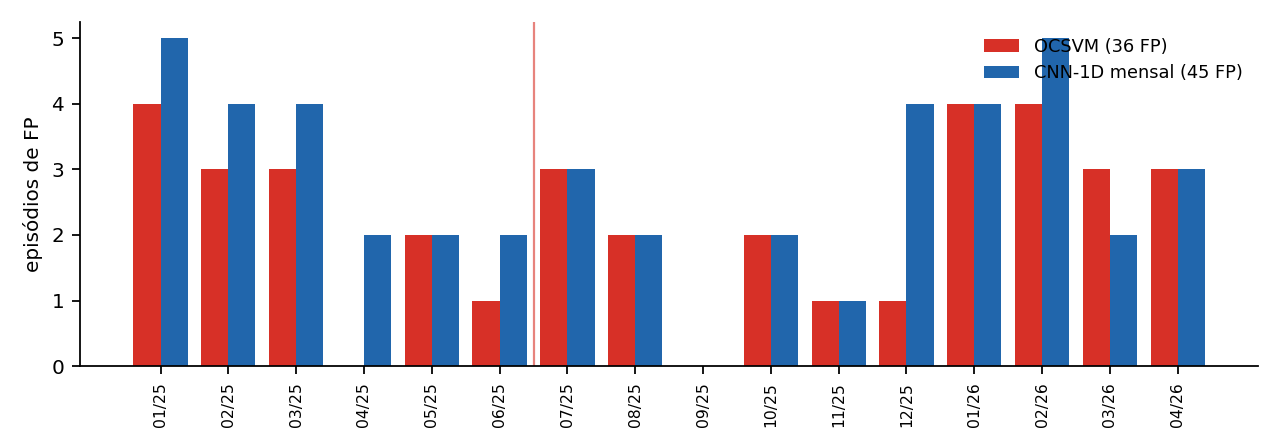
\includegraphics[width=0.9\textwidth]{fp_mensal.png}
\caption{Episódios de FP por mês, OCSVM $\times$ CNN-1D mensal (3 grupos). Linha vermelha: corte de 01/07/2025.}
\label{fig:fpmensal}
\end{figure}

\subsection{Série temporal dos dois modelos}

A Figura~\ref{fig:visao} mostra os 16 meses do recorte. Nos três painéis de cima aparecem o sinal original
(mediana horária, máquina em operação) e, embaixo de cada sinal, duas faixas: as horas com ponto anômalo da OCSVM
(vermelho) e do CNN-1D mensal (azul). O painel de baixo mostra os episódios da camada de decisão de cada modelo,
classificados pela régua, e as ativações dos dois alarmes recorrentes.

\begin{itemize}
  \item \textbf{Temperatura e óleo:} o CNN-1D acende mais que a OCSVM (1.210 contra 721 horas na temperatura, 321
        contra 118 no óleo).
  \item \textbf{Vibração:} o CNN-1D acende menos (1.315 contra 1.647~h).
  \item \textbf{Canal 4:} fica aceso 45,2\% do tempo de operação desde 01/2025.
  \item \textbf{Composição dos episódios:} trips, FP e inconclusivos aparecem nos mesmos lugares para os dois
        modelos, sempre perto de ativações de \tg{PI_6240319_AL} e \tg{PAL_6240315}.
\end{itemize}

\begin{figure}[p]
\centering
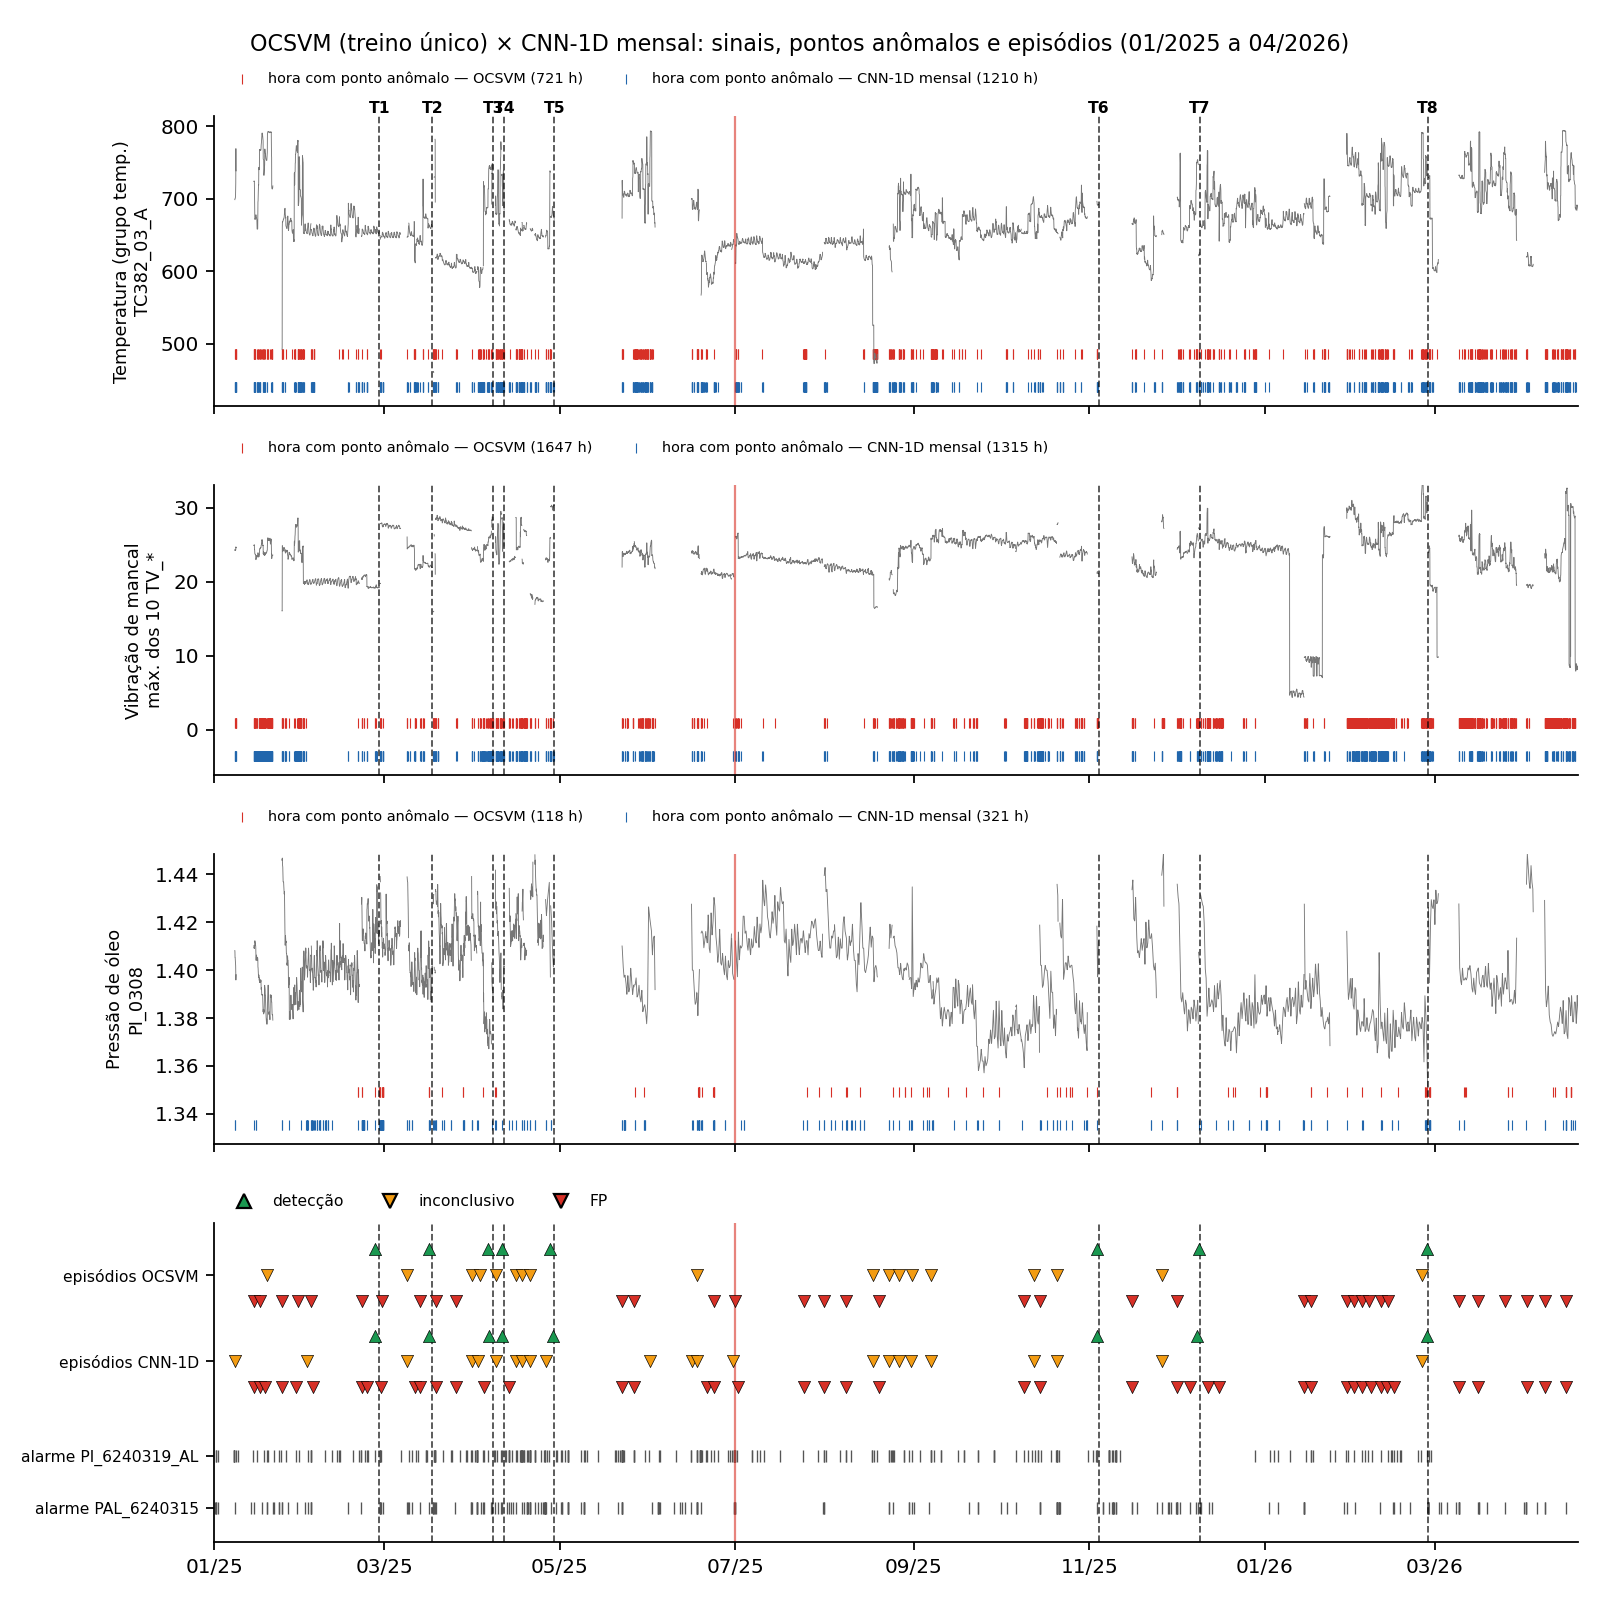
\includegraphics[width=\textwidth]{visao_conjunta.png}
\caption{OCSVM $\times$ CNN-1D mensal, 01/2025 a 04/2026. Sinal original e horas com ponto anômalo de cada modelo
(faixas vermelha e azul); episódios classificados pela régua (detecção em verde, inconclusivo em laranja,
FP em vermelho); alarmes de \tg{PI_6240319_AL} e \tg{PAL_6240315}. Tracejado: os 8 trips (T1 a T8). Linha vermelha:
corte fora da amostra. A vibração é o máximo dos 10 sensores \tg{TV_*}; as unidades são as do historiador.}
\label{fig:visao}
\end{figure}

\subsection{Os 8 trips em detalhe}

As Figuras~\ref{fig:t1} a~\ref{fig:t8} mostram cada trip numa janela de 60~h antes a 6~h depois. Cada figura tem
cinco painéis:
\begin{itemize}
  \item os três primeiros: os sinais, com faixas de pontos anômalos da OCSVM (vermelho) e do CNN-1D (azul);
  \item o quarto: o canal 4 aceso (cinza) e as ativações de alarme, com as tags de temperatura em laranja na
        metade de cima;
  \item o quinto: os episódios de cada modelo, coloridos pela classe.
\end{itemize}

\begin{figure}[H]\centering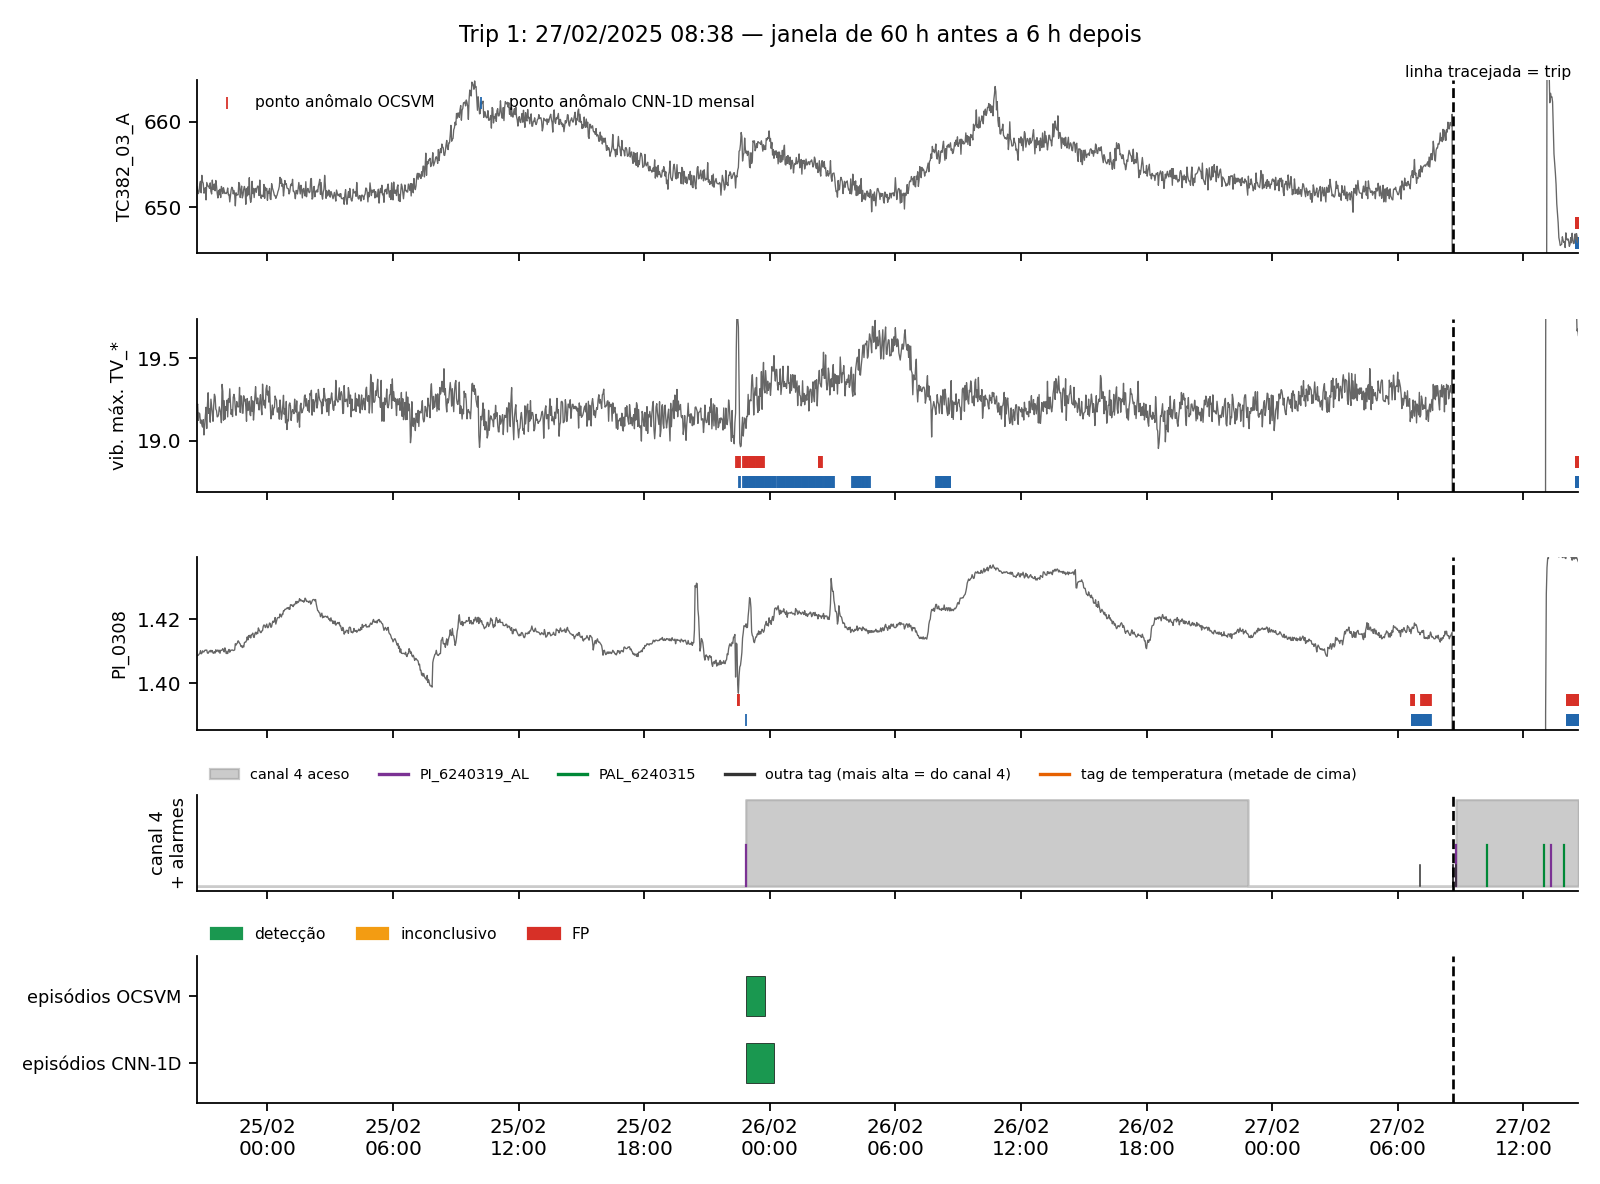
\includegraphics[width=0.92\textwidth]{zoom_trip_1.png}
\caption{T1, 27/02/2025: OCSVM e CNN-1D detectam com 33,8~h, ambos pela vibração junto do canal 4
(\tg{PI_6240319_AL}).}\label{fig:t1}\end{figure}

\begin{figure}[H]\centering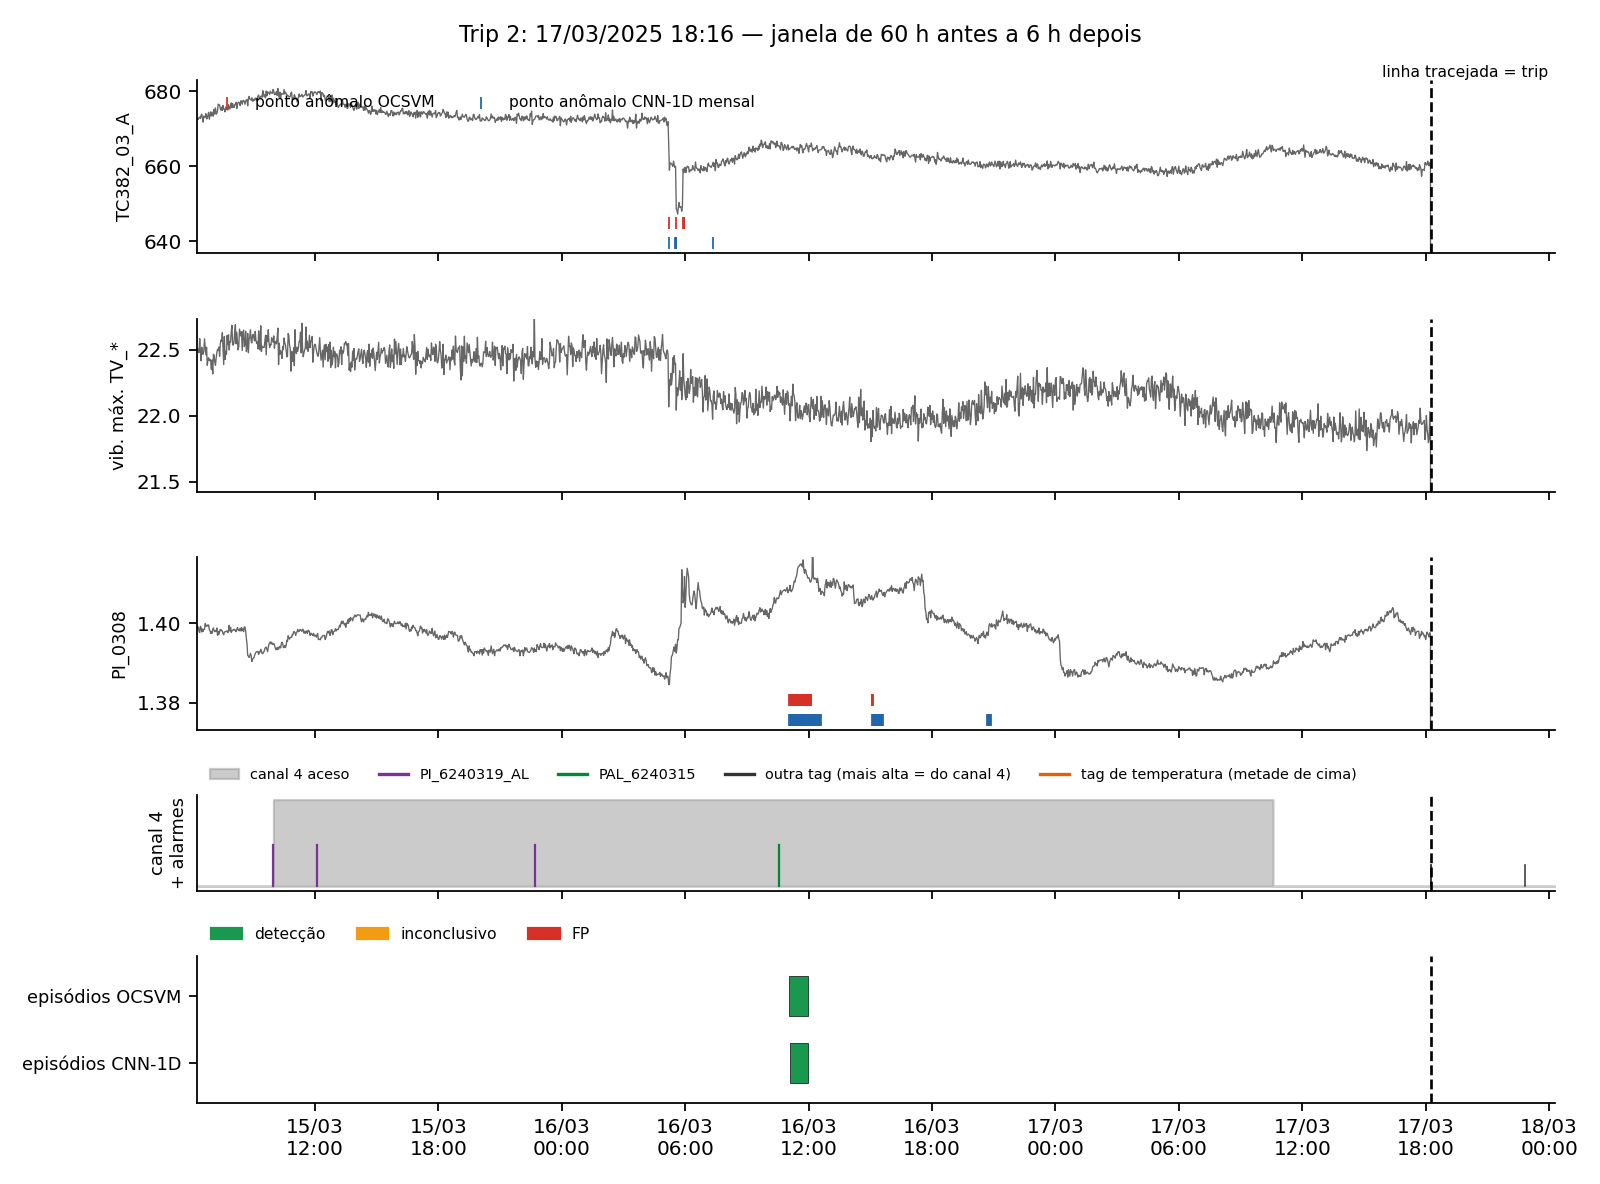
\includegraphics[width=0.92\textwidth]{zoom_trip_2.png}
\caption{T2, 17/03/2025: 31,2~h nos dois. O voto da OCSVM vem do óleo junto do canal 4.}\label{fig:t2}\end{figure}

\begin{figure}[H]\centering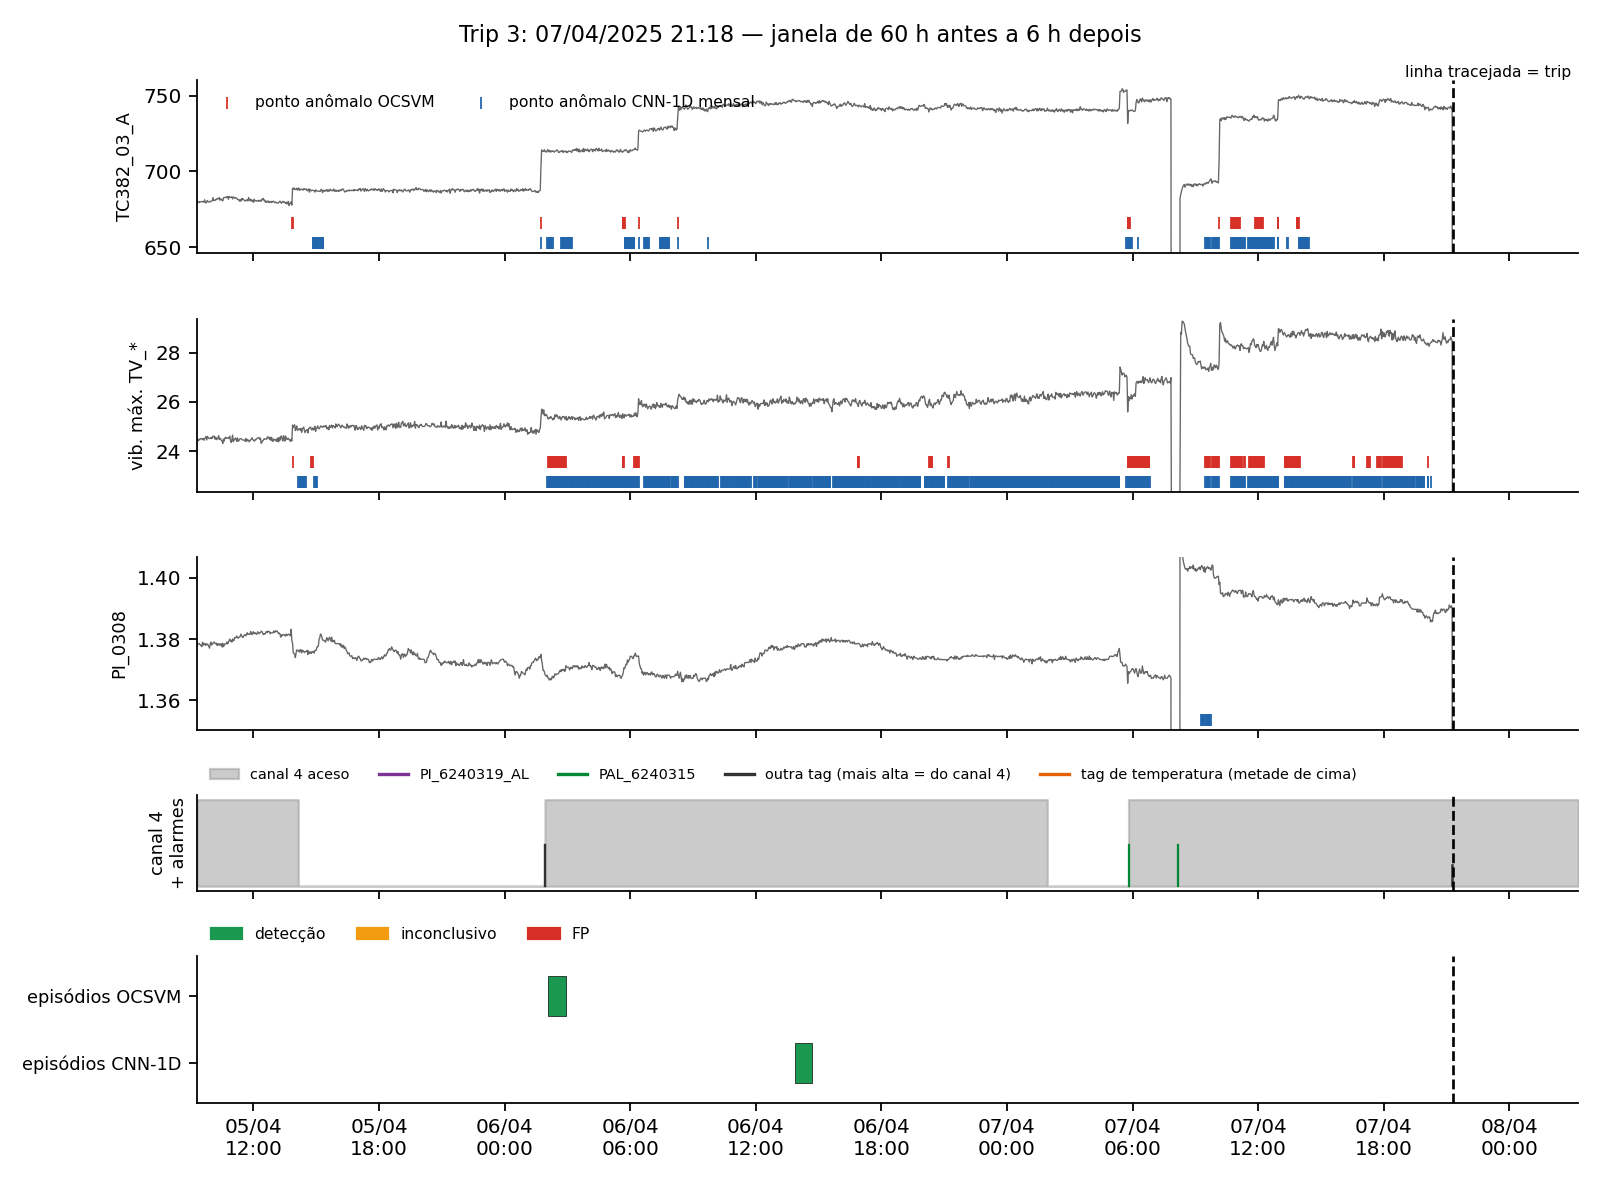
\includegraphics[width=0.92\textwidth]{zoom_trip_3.png}
\caption{T3, 07/04/2025: OCSVM com 43,2~h e CNN-1D com 31,4~h.}\label{fig:t3}\end{figure}

\begin{figure}[H]\centering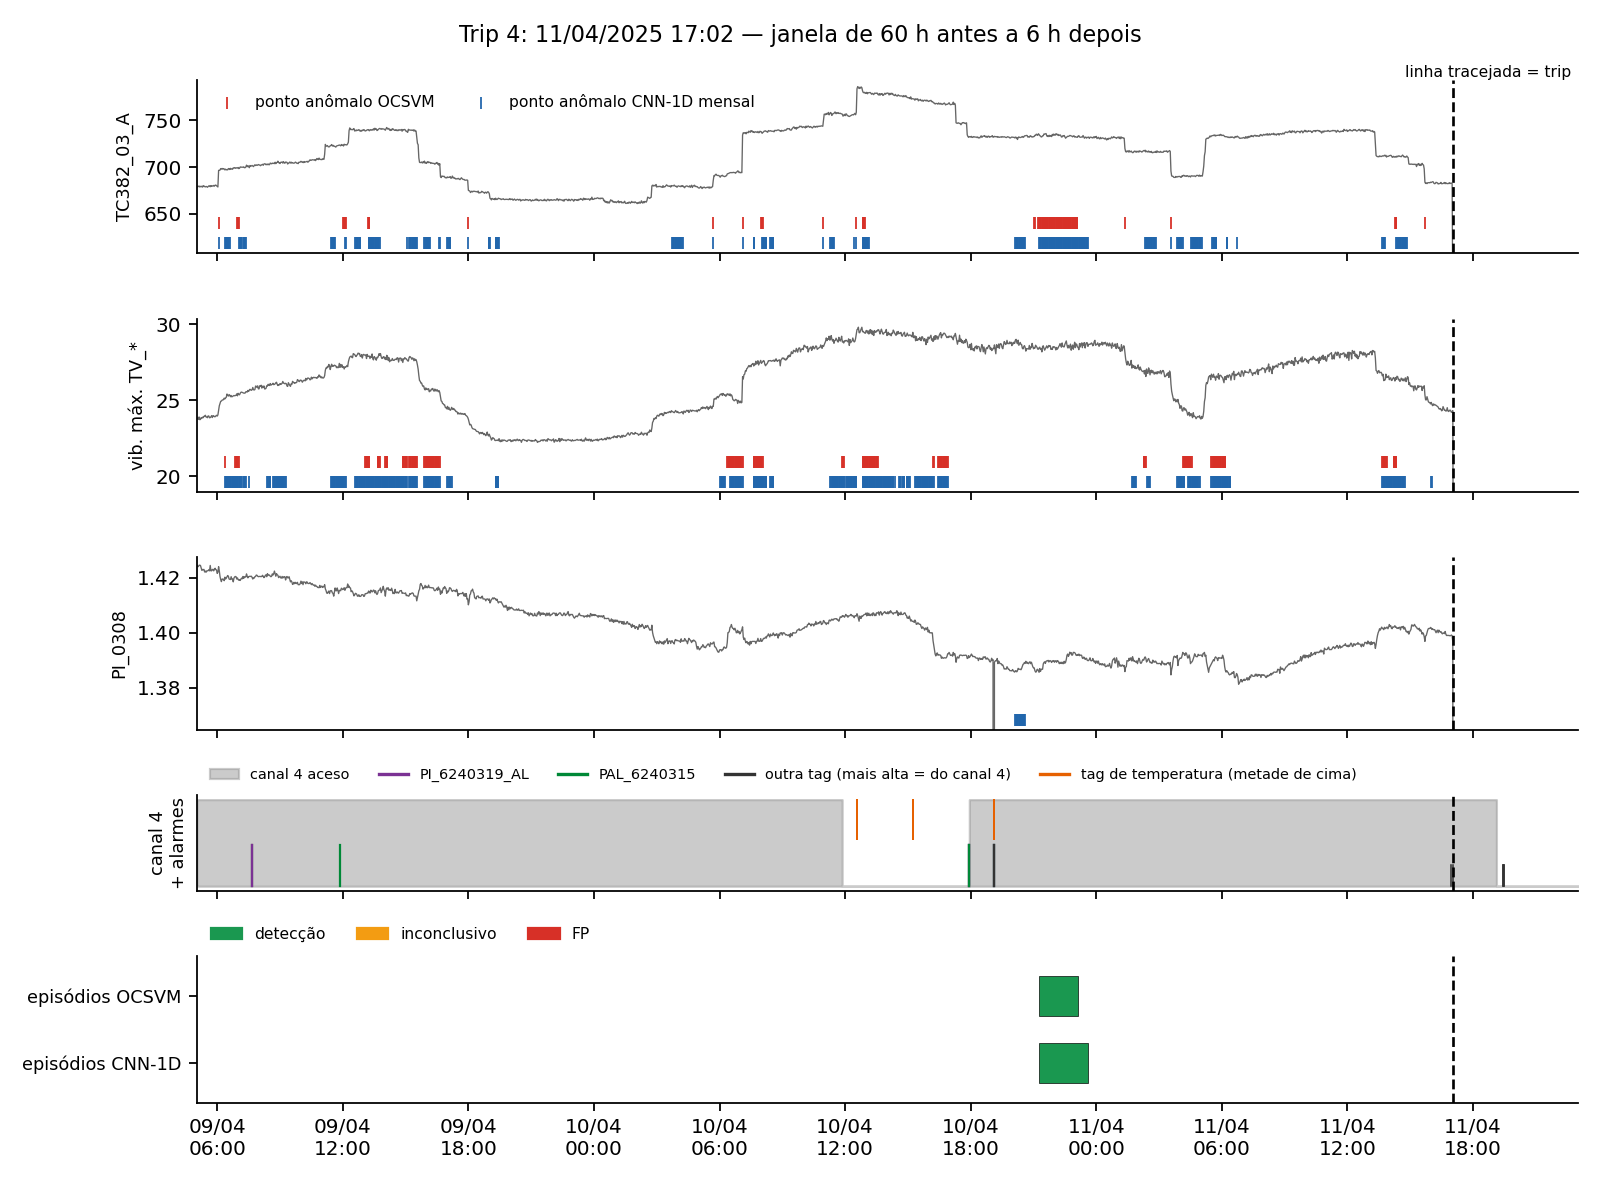
\includegraphics[width=0.92\textwidth]{zoom_trip_4.png}
\caption{T4, 11/04/2025: 19,8~h nos dois, pela temperatura junto do canal 4. Poucas horas antes da detecção, em 10/04, há uma
rajada de alarmes das tags de temperatura (laranja), a mesma assinatura que aparece em 5 FP (Seção~\ref{sec:rajada}).}
\label{fig:t4}\end{figure}

\begin{figure}[H]\centering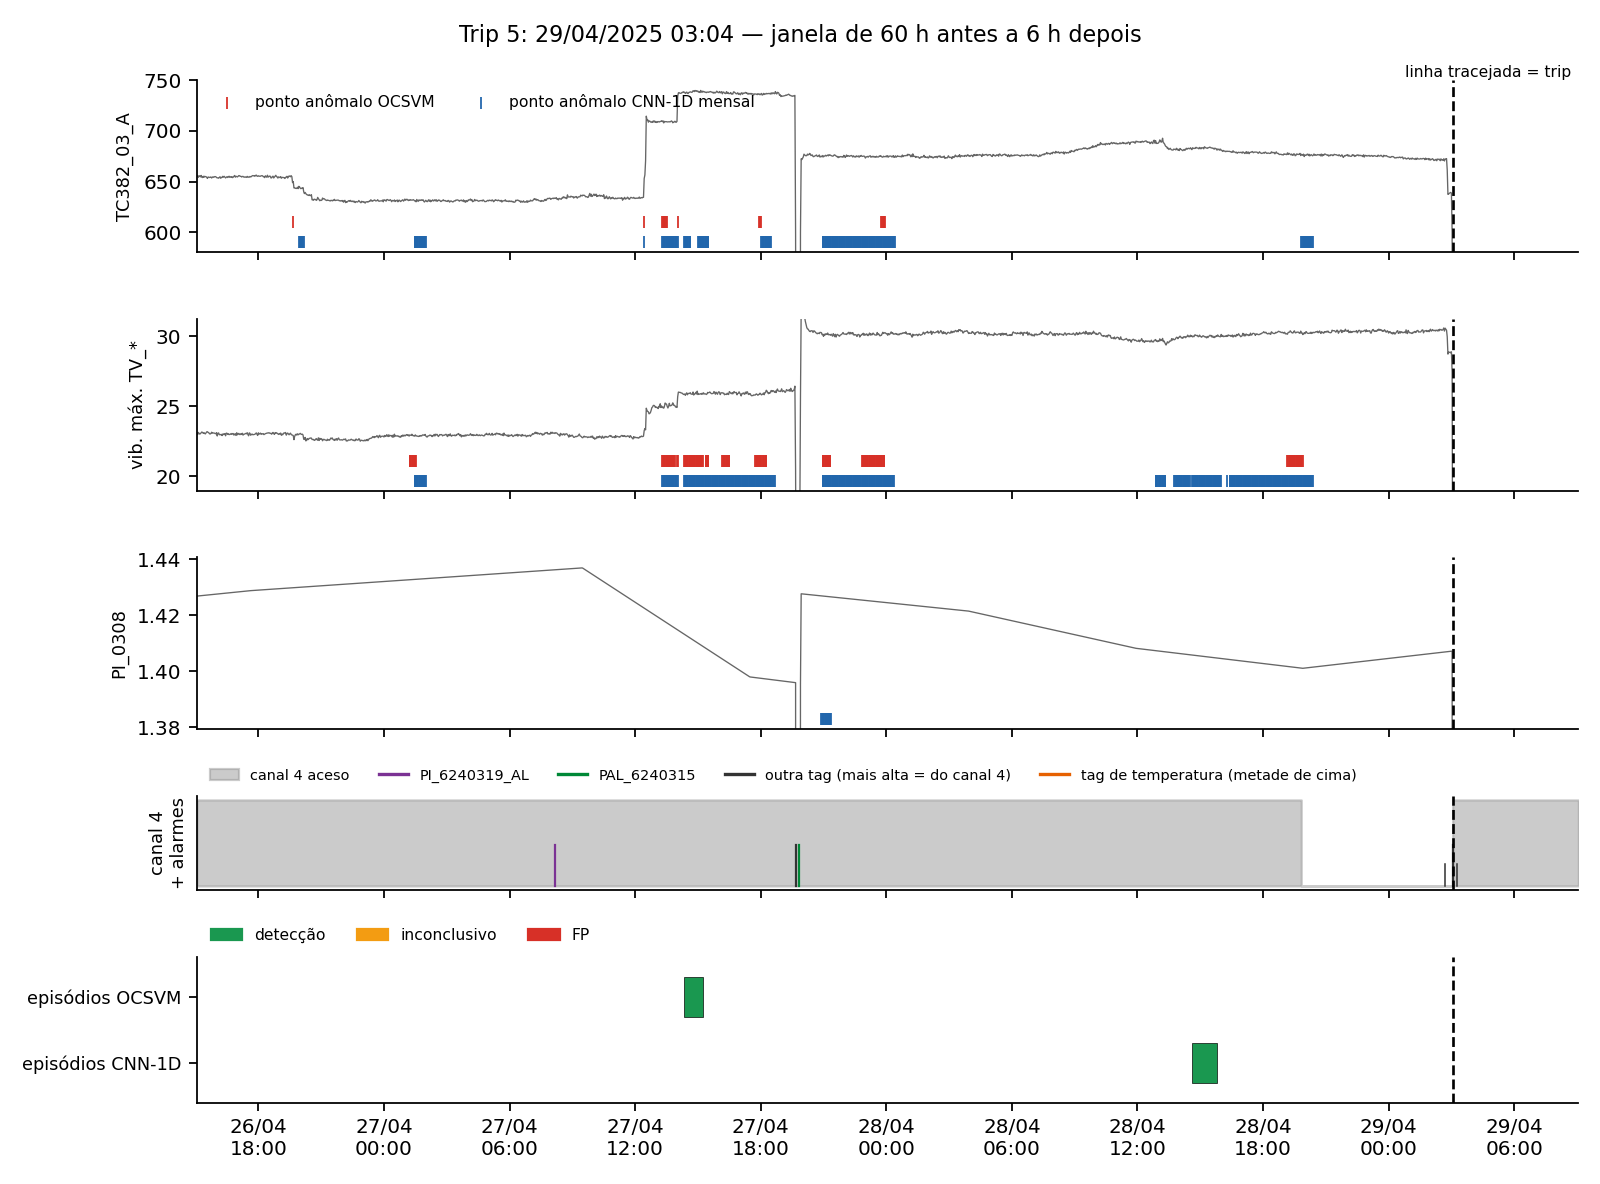
\includegraphics[width=0.92\textwidth]{zoom_trip_5.png}
\caption{T5, 29/04/2025: a OCSVM detecta com 36,7~h (vibração em 27/04 à tarde). O CNN-1D só fecha o voto em 28/04
à tarde, com 12,4~h.}\label{fig:t5}\end{figure}

\begin{figure}[H]\centering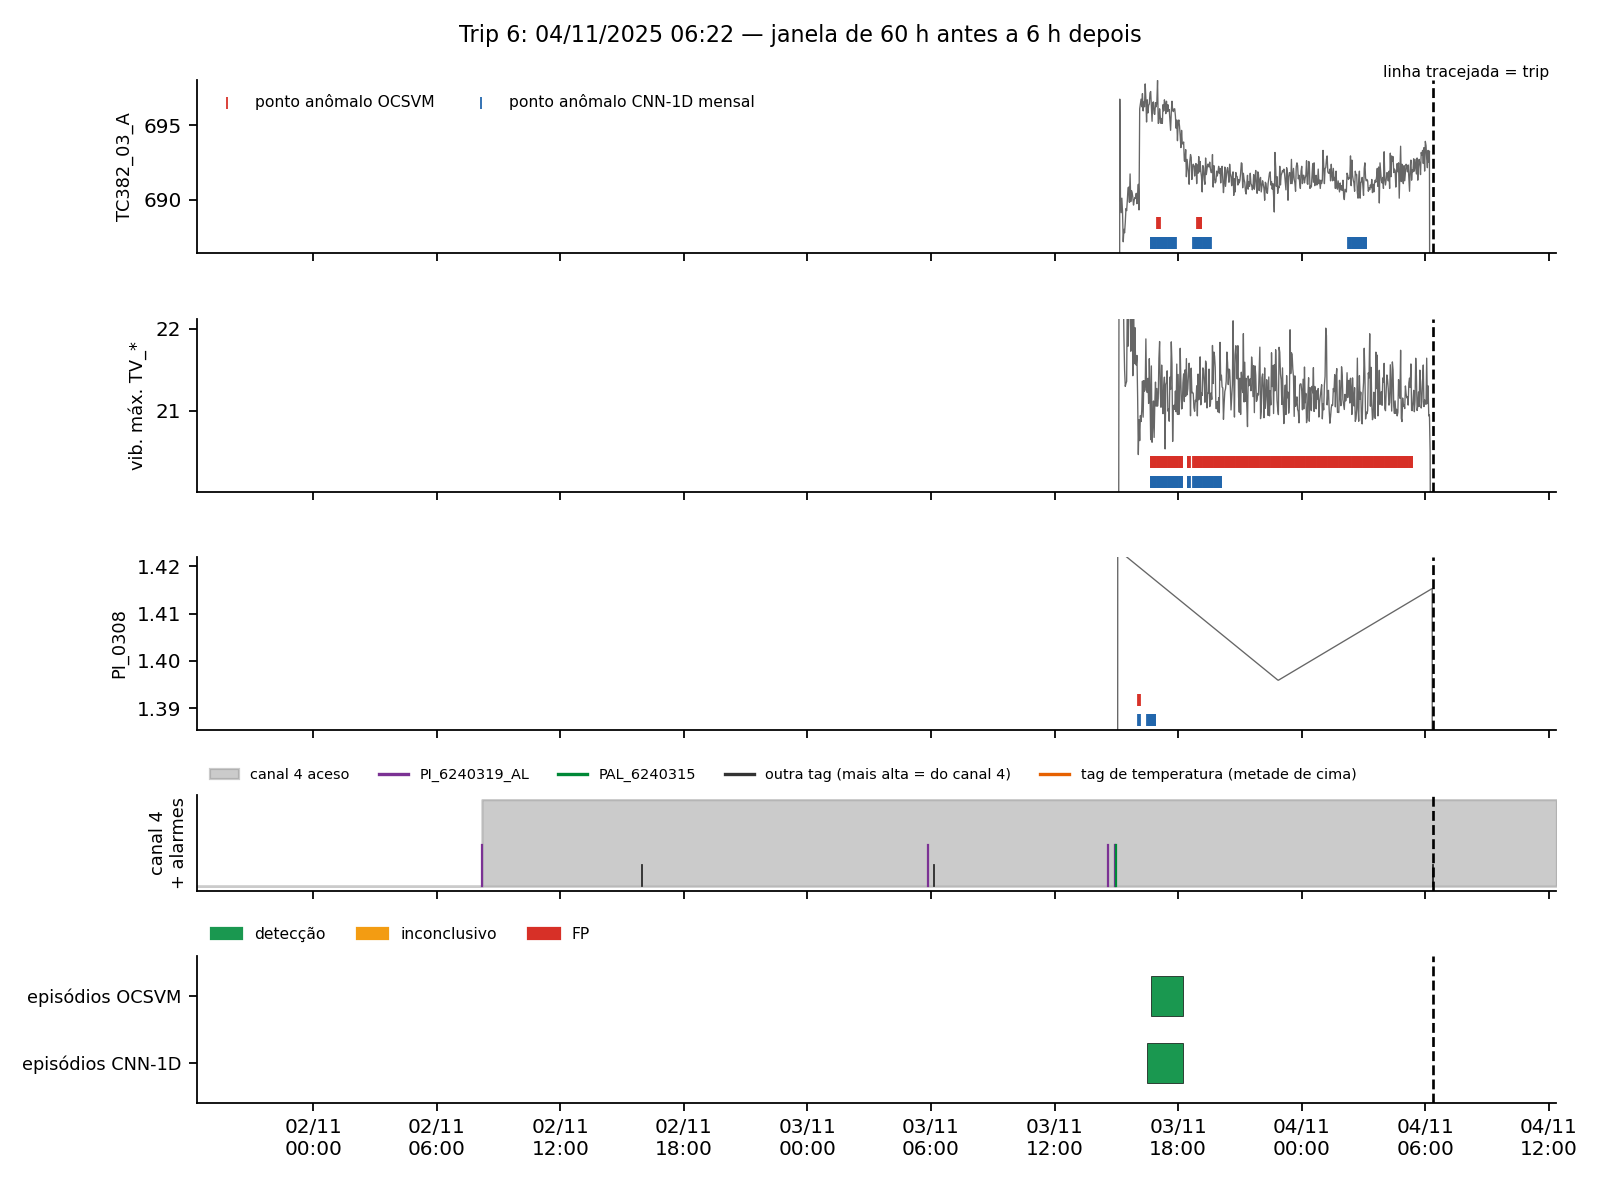
\includegraphics[width=0.92\textwidth]{zoom_trip_6.png}
\caption{T6, 04/11/2025: 13,7~h (OCSVM) e 13,9~h (CNN-1D).}\label{fig:t6}\end{figure}

\begin{figure}[H]\centering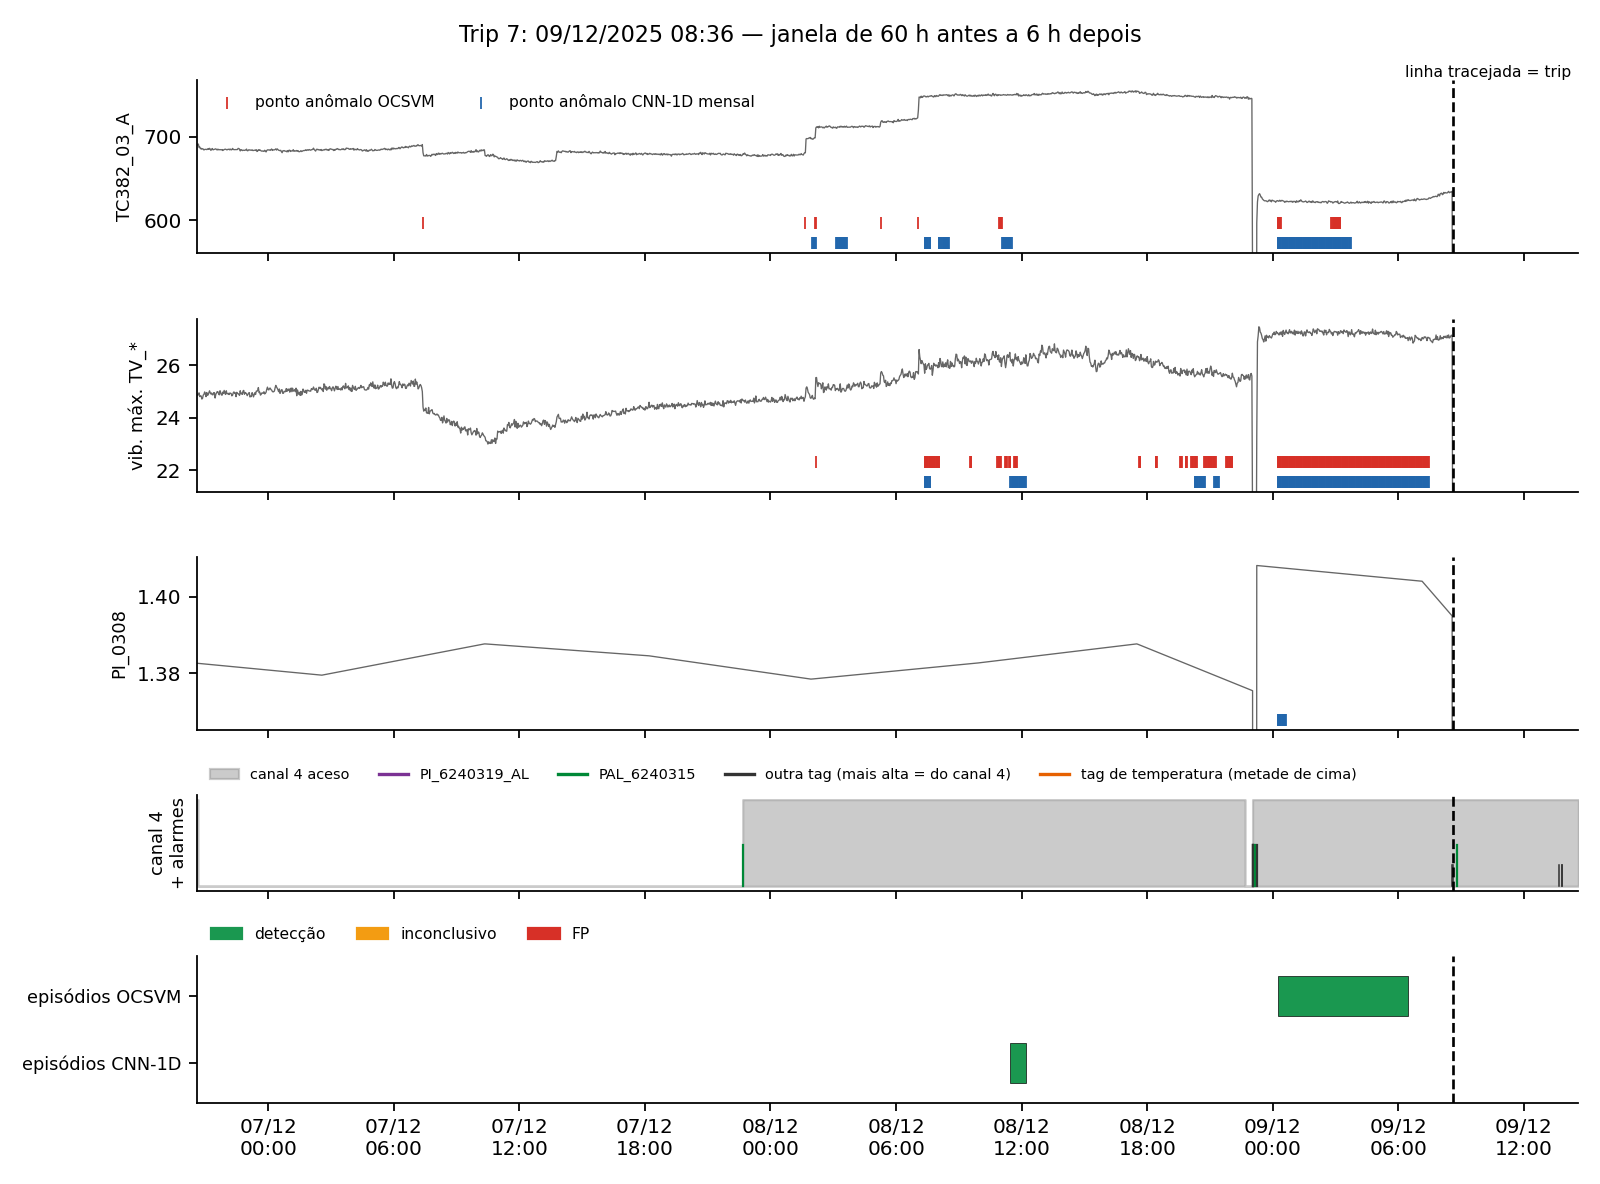
\includegraphics[width=0.92\textwidth]{zoom_trip_7.png}
\caption{T7, 09/12/2025: o CNN-1D detecta com 21,1~h, pela vibração e temperatura no fim da manhã de 08/12, quando
o canal 4 já estava aceso por \tg{PAL_6240315}. A OCSVM só fecha o voto depois da queda brusca do sinal na virada de 08 para 09/12
(8,4~h).}\label{fig:t7}\end{figure}

\begin{figure}[H]\centering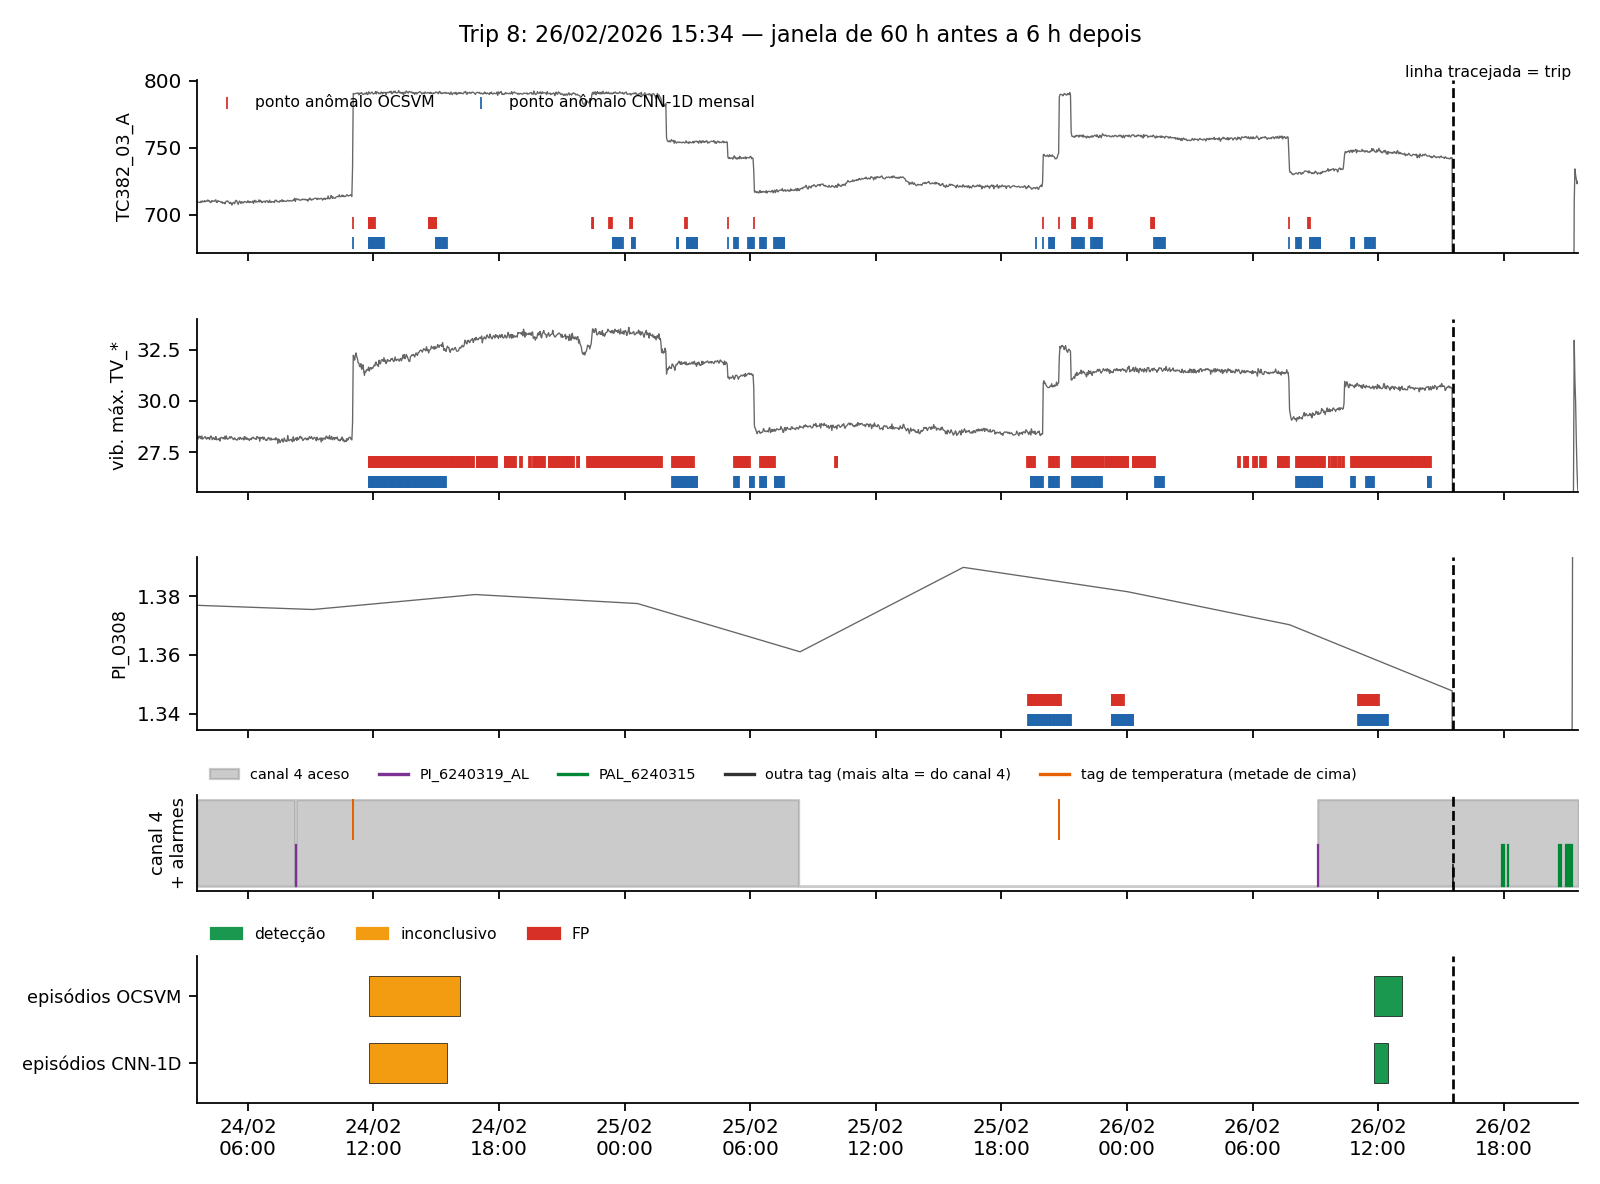
\includegraphics[width=0.92\textwidth]{zoom_trip_8.png}
\caption{T8, 26/02/2026: os dois modelos acendem desde 24/02. O primeiro episódio (24/02 11:47) começou 51,8~h antes
do trip, fora da janela de 48~h da régua, e por isso é inconclusivo. Ele dispara o refratário de 48~h, e a
``detecção'' nasce exatamente quando o refratário acaba (26/02 11:47), com 3,8~h. A antecedência curta do T8 é efeito
do refratário, não dos modelos.}\label{fig:t8}\end{figure}

\subsection{CNN-1D de vibração como canal extra (D2)}

Como o CNN-1D de vibração enxerga coisas que a OCSVM não vê (T7 com 21~h), ele foi testado também como canal
\emph{a mais}, sem substituir a OCSVM. O teste foi pré-registrado (commit \tg{37e0ca1}) e roda local, sem treino.

\begin{table}[H]
\centering\small
\caption{D2. A = 5º canal, voto $\geq 2$ de 5. B = a vibração só vota se a OCSVM e o CNN-1D acenderem juntos.}
\label{tab:d2}
\begin{tabular}{llllll}
\toprule
braço & trips & FP & FP/mês & trips fora & FP fora (FP/mês) \\
\midrule
produção & 8/8 & 36 & 3,051 & 3/3 & 23 (2,877) \\
A -- soma & 8/8 & 59 & 5,001 & 3/3 & 39 (4,878) \\
B -- confirmação & 8/8 & 34 & 2,882 & 3/3 & 21 (2,627) \\
\bottomrule
\end{tabular}
\end{table}

\begin{itemize}
  \item \textbf{Soma (A):} um canal a mais só soma votos, e o FP sobe 64\%.
  \item \textbf{Confirmação (B):} é segura, porque não perde trip e mantém as antecedências da produção. Mas corta
        só 6 a 9\% dos FP, porque as duas famílias quase sempre concordam na vibração.
  \item \textbf{Veredito:} nenhum dos dois passa.
\end{itemize}

%=====================================================================
\section{De onde vêm os pontos anômalos que não são trip}
\label{sec:diagnostico}
%=====================================================================

Depois dos placares, a pergunta passou a ser outra. Dá para eliminar, com regras depois do treino, os pontos
anômalos que não são trip nem alarme real? O cuidado necessário é que parte desses pontos pode ser \emph{resquício
de alarme de outro sensor}. Para responder, foi feito um diagnóstico só descritivo dos \textbf{62 episódios da
produção (OCSVM) desde 01/2025}: 8 detecções, 18 inconclusivos e 36 FP.

O diagnóstico mostrou que \textbf{quase todos os pontos anômalos já são, de fato, resto de alarme de outro sensor}.
As subseções a seguir detalham cada ponto.

\subsection{Origem: 61 dos 62 episódios nascem com o canal 4 aceso}

O voto $\geq 2$ quase nunca é fechado por dois modelos juntos, porque os três modelos coincidem só cerca de 1\% do
tempo. Na prática, o voto é \textbf{canal 4 + um modelo}. A Figura~\ref{fig:composicao} (esquerda) mostra quais
modelos estavam acesos em pelo menos metade de cada episódio:

\begin{itemize}
  \item \textbf{FP (36):} vibração sozinha em 23, temperatura em 4, óleo em 4, temperatura + vibração em 3, vibração
        + óleo em 2;
  \item \textbf{detecções (8):} vibração em 6, temperatura em 1 (T4), óleo em 1 (T2);
  \item \textbf{inconclusivos (18):} vibração em 11, temperatura + vibração em 4, temperatura em 2, óleo em 1.
\end{itemize}

Só um episódio (um inconclusivo de 26/08/2025) não tinha o canal 4 aceso. Com a máquina em operação, o canal 4 fica
aceso 45\% do tempo e a vibração da OCSVM, 12\%. Por isso, basta a vibração encostar numa janela de canal 4 para
virar alerta.

\begin{figure}[H]
\centering
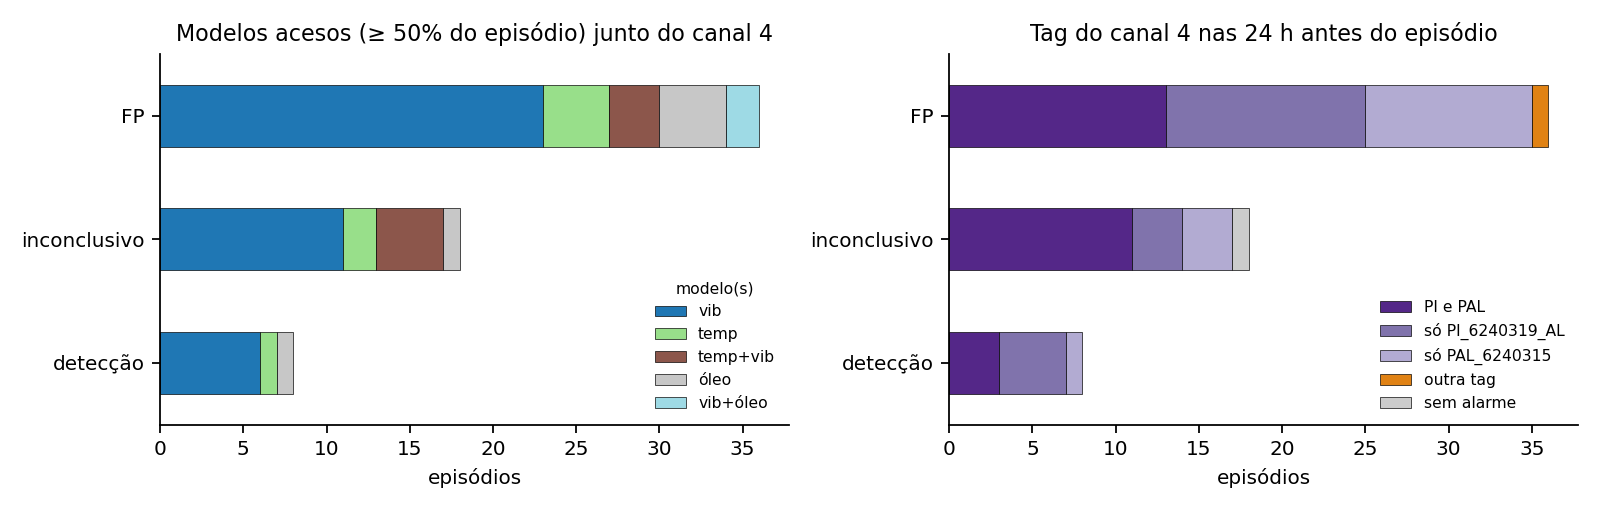
\includegraphics[width=\textwidth]{composicao_episodios.png}
\caption{Composição dos 62 episódios da produção desde 01/2025. Esquerda: modelo(s) aceso(s) em pelo menos metade do
episódio, junto do canal 4. Direita: qual das tags recorrentes acendeu o canal 4 nas 24~h antes do episódio.}
\label{fig:composicao}
\end{figure}

\subsection{O disparo é quase sempre \texttt{PI\_6240319\_AL} e/ou \texttt{PAL\_6240315}}

A Figura~\ref{fig:composicao} (direita) mostra a tag que acendeu o canal 4 nas 24~h antes de cada episódio:

\begin{itemize}
  \item \textbf{FP:} as duas tags em 13, só \tg{PI_6240319_AL} em 12, só \tg{PAL_6240315} em 10, outra tag em 1;
  \item \textbf{detecções:} as duas em 3, só \tg{PI_6240319_AL} em 4, só \tg{PAL_6240315} em 1;
  \item \textbf{inconclusivos:} as duas em 11, só \tg{PI_6240319_AL} em 3, só \tg{PAL_6240315} em 3, sem alarme
        em 1.
\end{itemize}

No total, \textbf{60 dos 62 episódios} têm uma dessas duas tags no gatilho. Isso inclui os 8 trips.

\subsection{Essas duas tags são os alarmes recorrentes sem trip}

As duas são as tags \textbf{mais recorrentes de todo o catálogo} (Figura~\ref{fig:recorrencia} e
Tabela~\ref{tab:recorrencia}). Desde 07/2024, \tg{PI_6240319_AL} foi a alarme 409 vezes e \tg{PAL_6240315}, 326.
Só 27 e 31 dessas ativações caem na janela de 48~h antes a 24~h depois de algum trip: 58 de 735, \textbf{cerca de
8\%}. Em mais de 90\% das vezes, o alarme toca e não vem trip nenhum.

\begin{figure}[H]
\centering
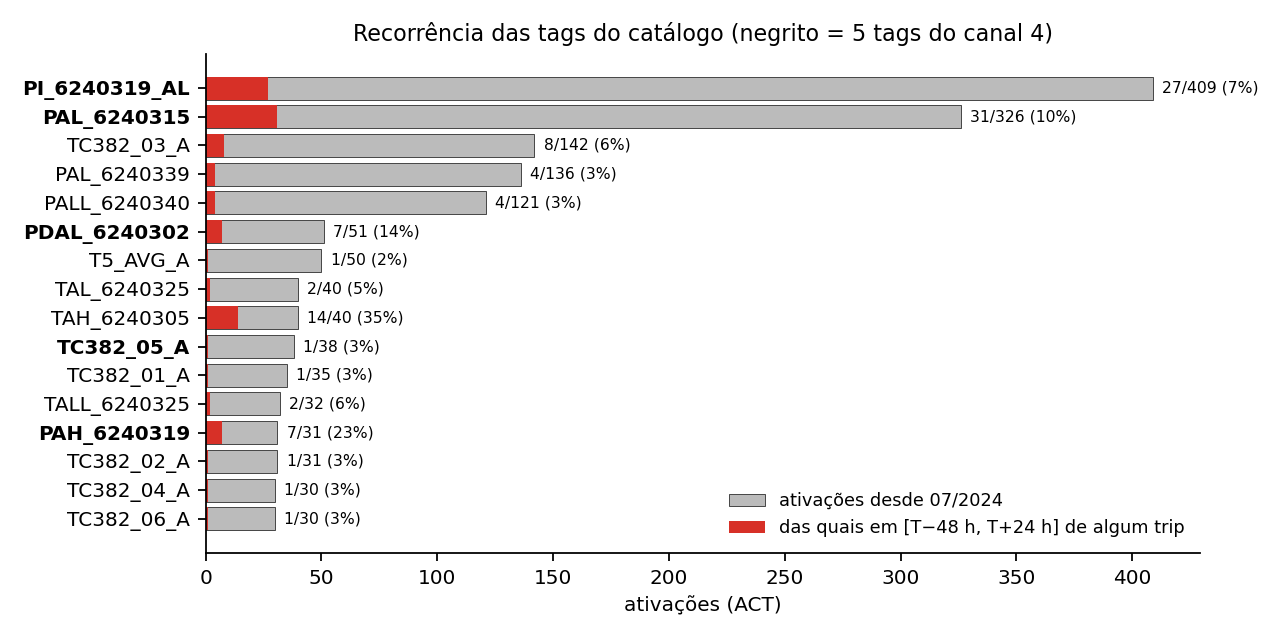
\includegraphics[width=0.9\textwidth]{recorrencia_tags.png}
\caption{Ativações de cada tag desde 07/2024 (cinza) e quantas caem em $[T-48\,\text{h},\,T+24\,\text{h}]$ de algum
trip (vermelho). Em negrito, as 5 tags do canal 4.}
\label{fig:recorrencia}
\end{figure}

\begin{table}[H]
\centering\small
\caption{Recorrência das 16 tags mais frequentes desde 07/2024.}
\label{tab:recorrencia}
\begin{tabular}{lllll}
\toprule
tag & ativações & perto de trip & \% perto de trip & canal 4 \\
\midrule
PI\_6240319\_AL & 409 & 27 & 7 & sim \\
PAL\_6240315 & 326 & 31 & 10 & sim \\
TC382\_03\_A & 142 & 8 & 6 &  \\
PAL\_6240339 & 136 & 4 & 3 &  \\
PALL\_6240340 & 121 & 4 & 3 &  \\
PDAL\_6240302 & 51 & 7 & 14 & sim \\
T5\_AVG\_A & 50 & 1 & 2 &  \\
TAL\_6240325 & 40 & 2 & 5 &  \\
TAH\_6240305 & 40 & 14 & 35 &  \\
TC382\_05\_A & 38 & 1 & 3 & sim \\
TC382\_01\_A & 35 & 1 & 3 &  \\
TALL\_6240325 & 32 & 2 & 6 &  \\
PAH\_6240319 & 31 & 7 & 23 & sim \\
TC382\_02\_A & 31 & 1 & 3 &  \\
TC382\_04\_A & 30 & 1 & 3 &  \\
TC382\_06\_A & 30 & 1 & 3 &  \\
\bottomrule
\end{tabular}

\end{table}

A Figura~\ref{fig:chattering} mostra o padrão típico. Entre 31/01 e 13/02/2026, a vibração da OCSVM ficou acesa
63\% do tempo de operação. Cada nova ativação de \tg{PI_6240319_AL} reacende o canal 4 por 24~h e gera mais um
episódio de FP, o que dá cinco FP em duas semanas sem trip. No mesmo trecho, o CNN-1D de vibração ficou aceso 25\% do
tempo e gerou o mesmo número de FP.

\begin{figure}[H]
\centering
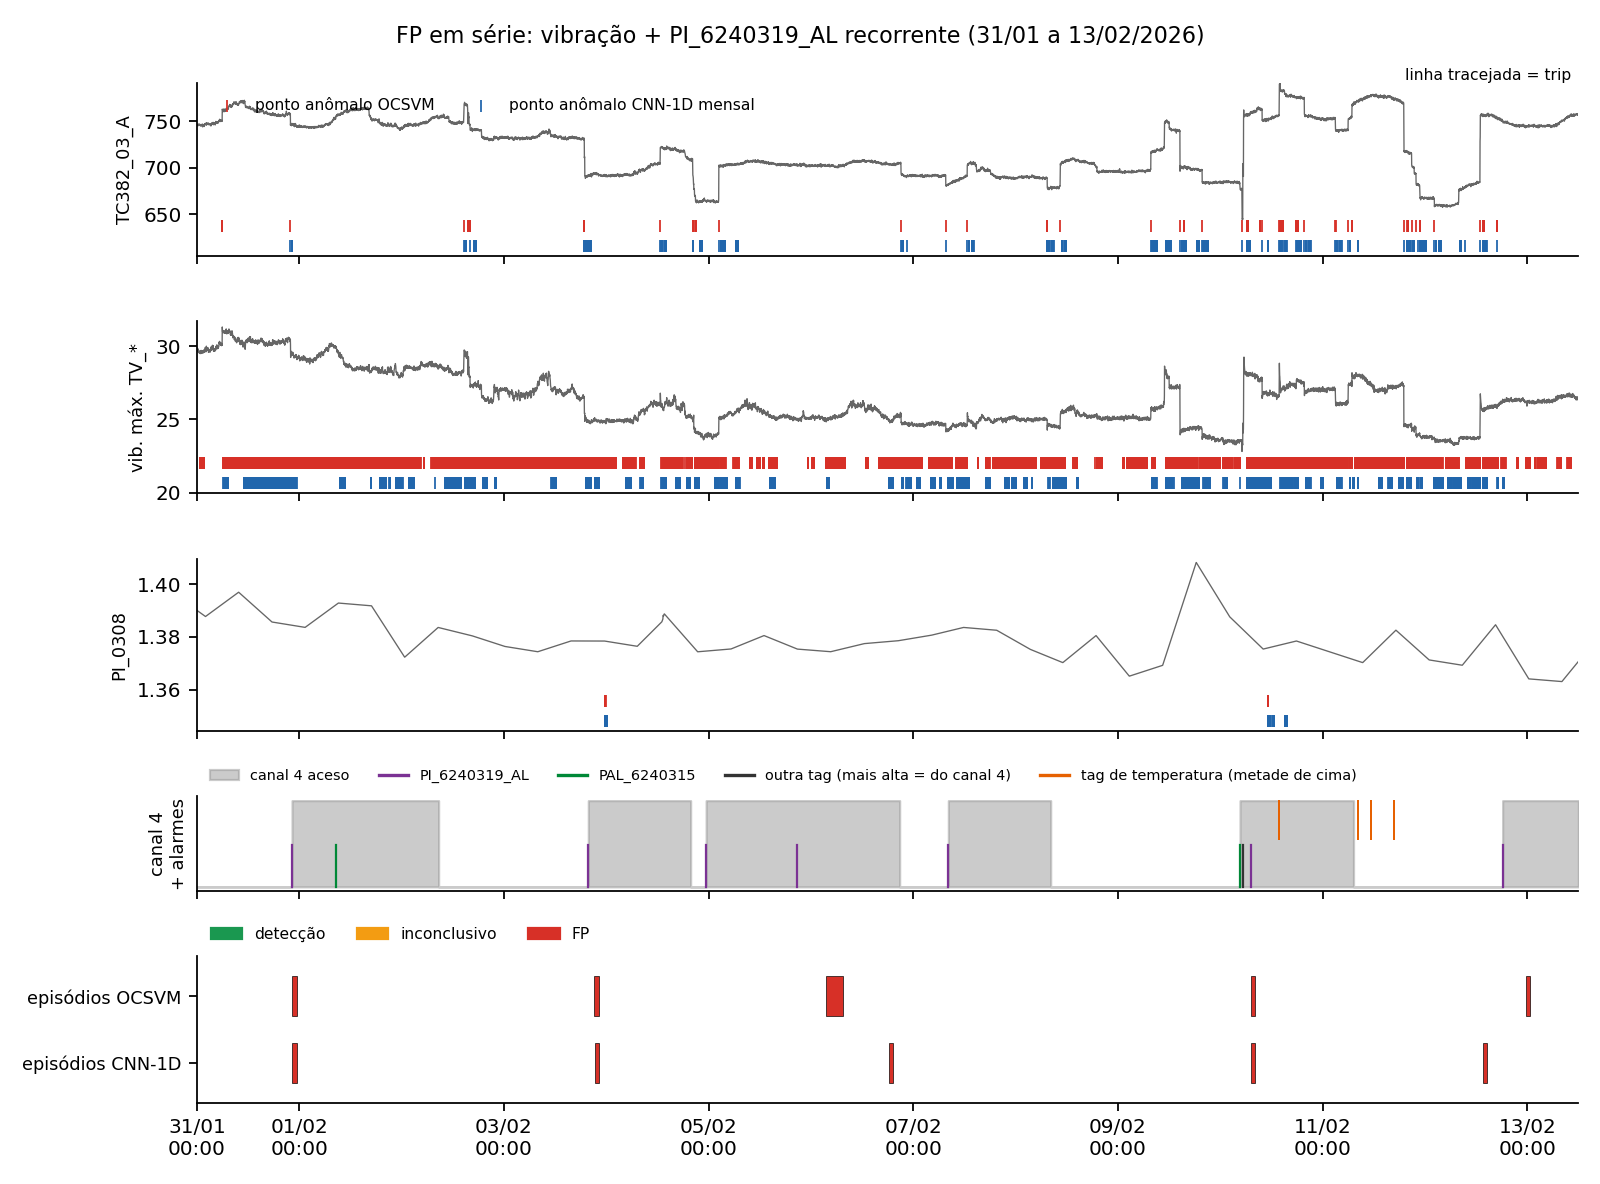
\includegraphics[width=0.92\textwidth]{zoom_fp_chattering.png}
\caption{FP em série, de 31/01 a 13/02/2026: vibração acesa quase o tempo todo e o canal 4 reaceso a cada ativação
de \tg{PI_6240319_AL} (roxo).}
\label{fig:chattering}
\end{figure}

\subsection{O problema: os 8 trips nascem das mesmas tags}

Se as duas tags só gerassem FP, bastaria tirá-las do canal 4. Mas os 8 trips têm a \textbf{mesma composição}:
canal 4 aceso por essas tags e um modelo, quase sempre a vibração (6 dos 8). Por isso, cortar por tag sempre mata
trips. Os testes anteriores mostraram isso:

\begin{itemize}
  \item \textbf{A3 (LOEO da camada de decisão):} só \tg{PI_6240319_AL} é indispensável (sem ela, 6/8). T1 e T8 só
        são pegos com ela. Escolhendo tags e janela sem o trip avaliado, o resultado cai para 5/8.
  \item \textbf{B1 (debounce do chattering):} contar a ativação só depois de um silêncio de até 24~h não perde trip,
        mas corta no máximo 0,14 FP/mês. O canal 4 fica aceso por alarmes espaçados de horas, não por rajadas.
  \item \textbf{A2 (nulo de acaso):} sem o canal 4, a pipeline faz 0/8. Com ele sempre ligado, 8/8 a 4,67 FP/mês. O
        canal 4 é o filtro de custo, e só funciona alinhado aos trips.
\end{itemize}

\subsection{Quando há parada real depois, o episódio já não conta como FP}

Uma anomalia seguida de parada real ($\geq 2$~h em até 48~h) pode ser um evento físico verdadeiro sem rótulo. Esses
casos já saem da conta de FP: a régua os classifica como \textbf{inconclusivos}, que são \textbf{18} desde 01/2025
na OCSVM e 23 no CNN-1D. A Figura~\ref{fig:inconclusivo} mostra um exemplo. Os 36 FP restantes são os que
\emph{não} têm trip nem parada em seguida.

\begin{figure}[H]
\centering
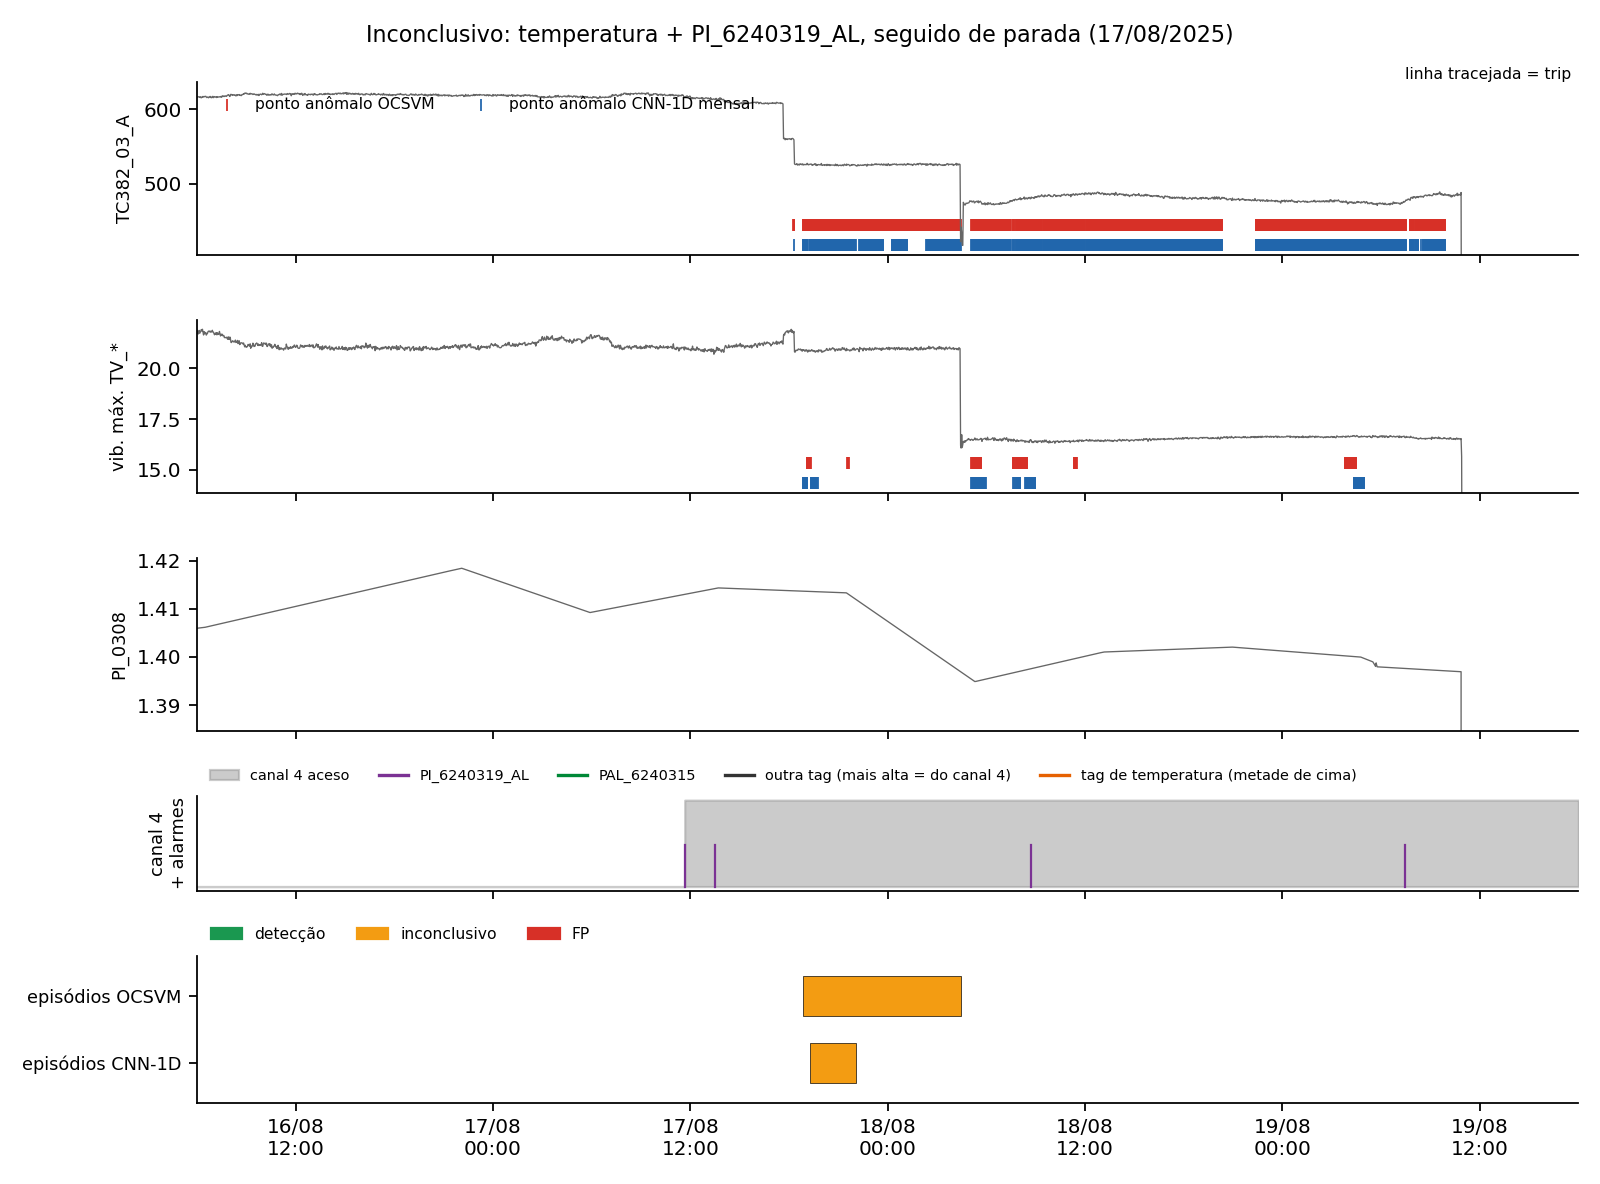
\includegraphics[width=0.92\textwidth]{zoom_inconclusivo.png}
\caption{Inconclusivo de 17/08/2025: temperatura acesa com \tg{PI_6240319_AL}, seguida de parada da máquina. Não
conta como FP.}
\label{fig:inconclusivo}
\end{figure}

\subsection{Duas hipóteses já descartadas}

\begin{itemize}
  \item \textbf{B5 (FP como ``alarme antecipado''):} a hipótese era que o FP antecede um alarme novo do catálogo. Os
        FP não antecipam alarmes novos além do acaso: 14 de 42 (33\%) contra 47,6\% esperados; sem as 5 tags do
        canal 4, 17\% contra 15,6\%.
  \item \textbf{B3 (exigir 2 modelos juntos):} a prioridade ``ALTA só com 2 OCSVM juntas'' rebaixa exatamente os 5
        trips de 2025 (3/8 em ALTA). Fora da amostra, ela pôs os 3 trips em ALTA e rebaixou 52\% dos FP. Fica como
        hipótese para dados novos.
\end{itemize}

\subsection{Um achado novo: rajadas de alarmes de temperatura}
\label{sec:rajada}

O diagnóstico mostrou uma assinatura que não tinha sido olhada: \textbf{rajadas simultâneas de alarmes de todas as
tags de temperatura}. Em 24/07/2025 (Figura~\ref{fig:rajada}), \tg{TC382_01_A} a \tg{TC382_06_A},
\tg{TI_6240315}, \tg{TI_6240317} e \tg{T5_AVG_A} foram a alarme \emph{no mesmo segundo} (16:14:37), e
\tg{PI_6240319_AL} veio 56~s depois. O sinal de temperatura, porém, não mostra nada fora do comum. Tem cara de evento
de instrumentação ou do sistema de alarmes, e não de processo.

Desde 07/2024 houve 19 rajadas desse tipo (5 ou mais tags de temperatura em 10~min). No recorte, elas aparecem perto
de 5 FP, 1 inconclusivo e \textbf{1 detecção (T4)}. Uma regra que suprimisse alertas perto de rajadas mataria o T4.
Como o achado veio dos mesmos dados, qualquer regra baseada nele seria ajustada a posteriori.

\begin{figure}[H]
\centering
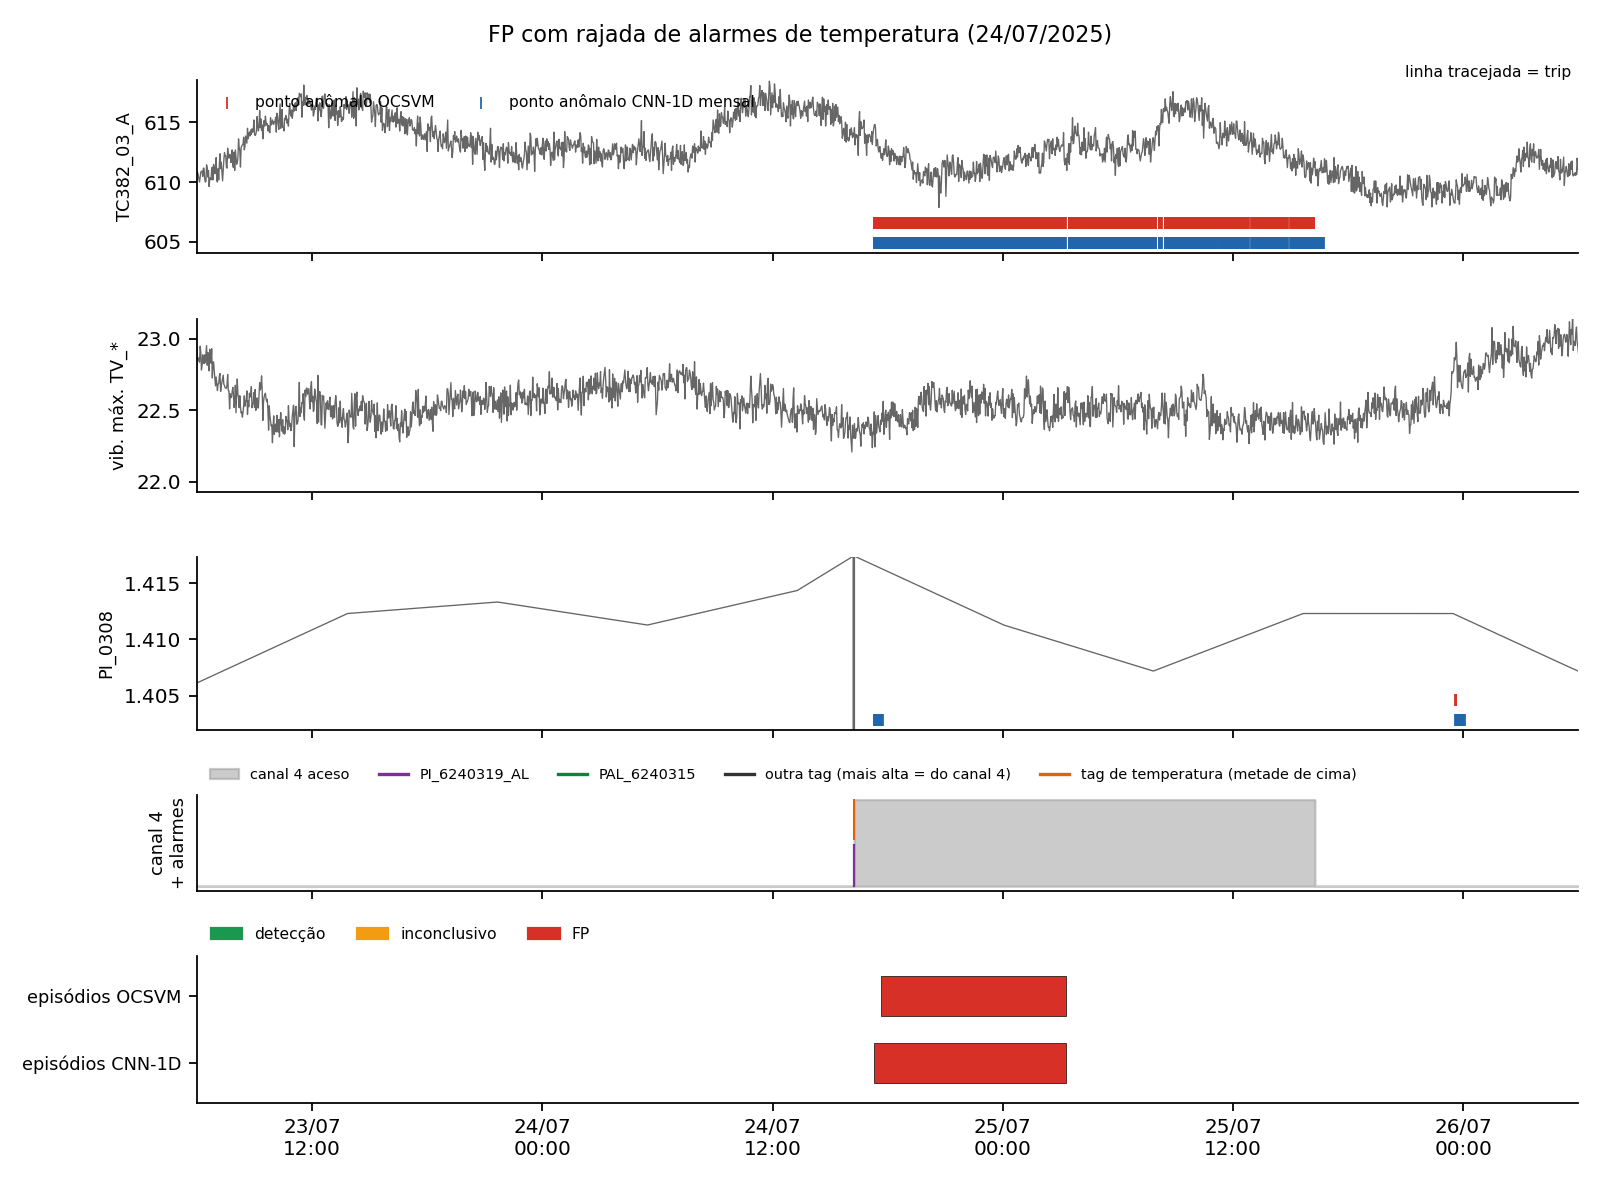
\includegraphics[width=0.92\textwidth]{zoom_fp_rajada.png}
\caption{FP de 24/07/2025: rajada de 9 alarmes de temperatura no mesmo segundo (laranja) e \tg{PI_6240319_AL} logo
depois. Os dois modelos marcam a temperatura por cerca de 10~h, sem mudança visível no sinal.}
\label{fig:rajada}
\end{figure}

\begin{figure}[H]
\centering
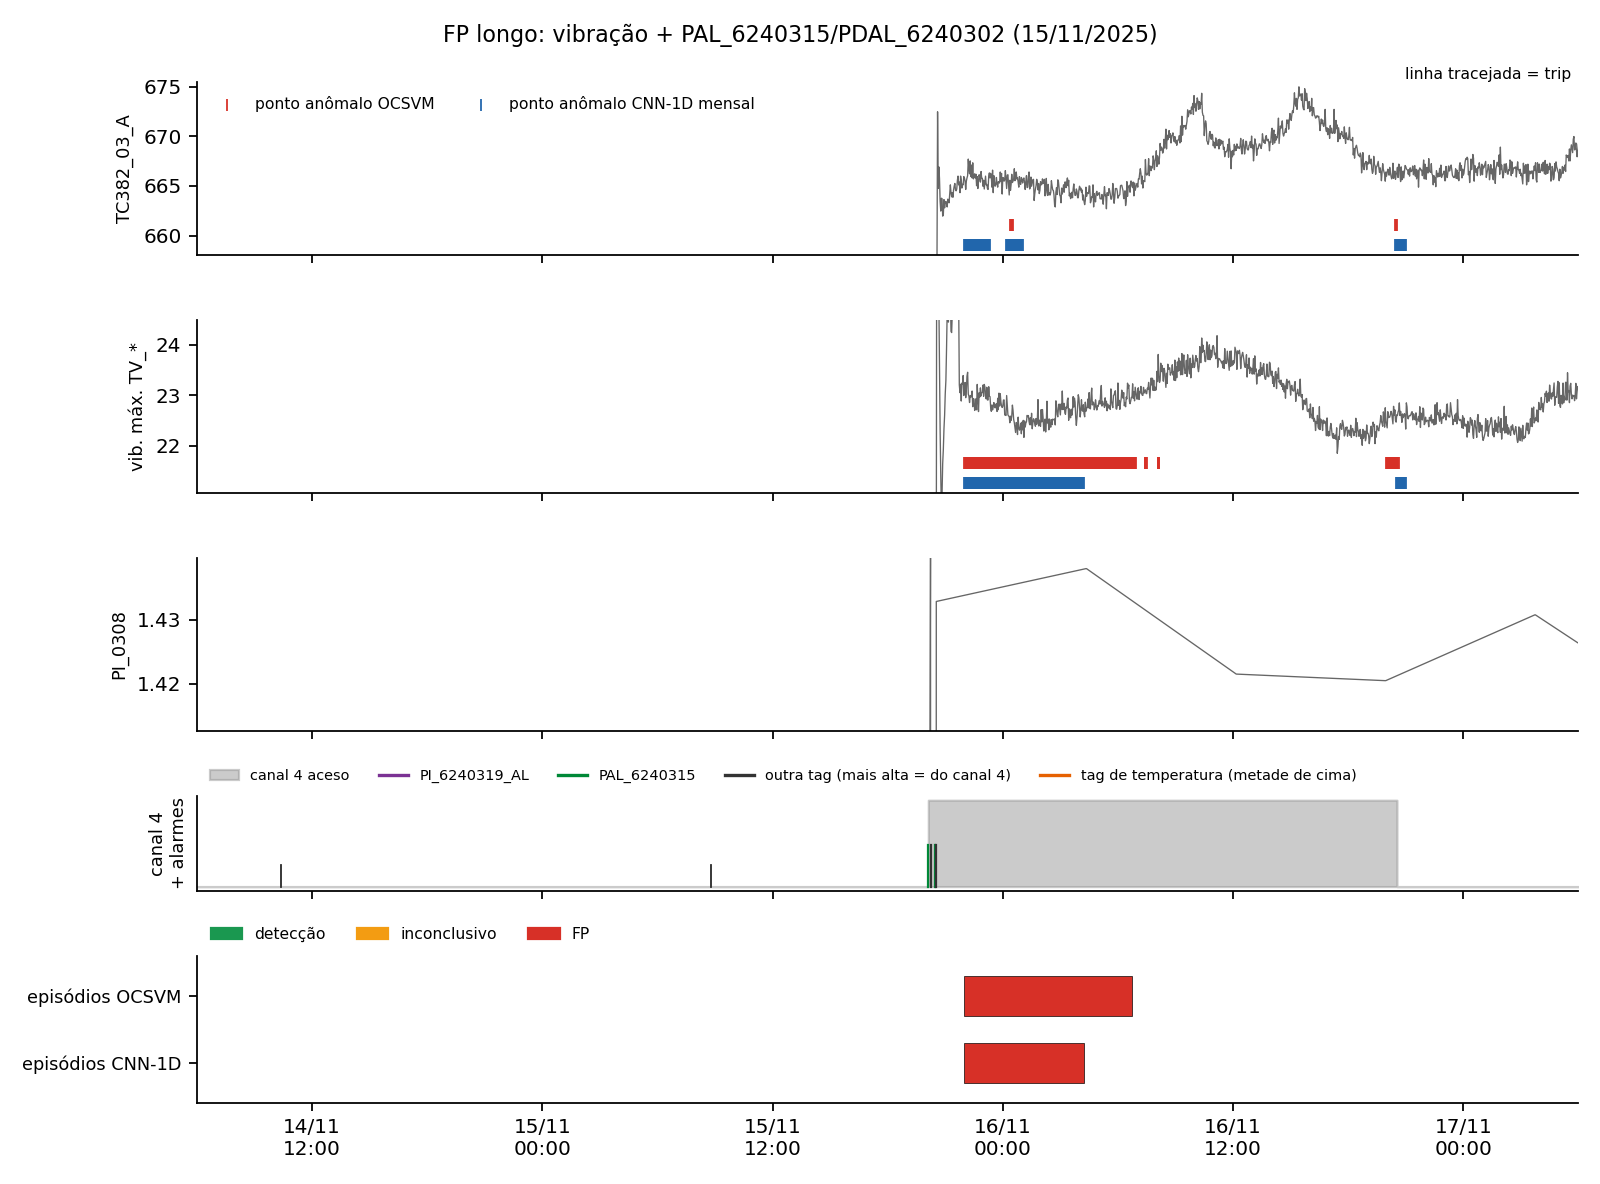
\includegraphics[width=0.92\textwidth]{zoom_fp_longo.png}
\caption{FP longo de 15/11/2025 (8,7~h): vibração com o canal 4 aceso por \tg{PAL_6240315} e \tg{PDAL_6240302}.}
\label{fig:fplongo}
\end{figure}

\subsection{Conclusão do diagnóstico}

Com alarmes, canais e votos, \textbf{a separação entre FP e trip está esgotada nesses dados}. Os pontos anômalos
que não são trip são, na maioria, resquício de alarmes recorrentes. Os trips são resquício dos \emph{mesmos}
alarmes, e mais regras do mesmo tipo trocam FP por trips perdidos. O que falta não é regra. São dados que
distingam as duas situações.

%=====================================================================
\section{Problemas dos dados atuais}
\label{sec:problemas}
%=====================================================================

\begin{enumerate}
  \item \textbf{Poucos eventos.} São só 8 trips em 22 meses, 5 deles dentro do período de treino da OCSVM e 3 fora.
        Com 3 trips fora da amostra, qualquer diferença de um evento muda o veredito. Nenhum teste distingue
        ``melhor'' de ``sorte'' com essa contagem.
  \item \textbf{As regras foram escolhidas olhando os mesmos trips.} O filtro de 45~min, a janela de 24~h, as 5 tags e
        o refratário de 48~h foram ajustados nos 8 trips. Validação cruzada deixando um trip de fora (A3) cai para
        5/8.
  \item \textbf{Resultado frágil ao corte do treino.} Mudar o corte de 01/07 para 01/05/2025 derruba a OCSVM para 4/8
        (A4). O AutoML da vibração troca de limiar e o canal quase se cala.
  \item \textbf{Paradas sem rótulo de causa.} Desde 01/2025 houve 66 paradas de 2~h ou mais, e só 8 são trips
        curados. As demais podem ser paradas programadas, manobras ou falhas não catalogadas. A régua as trata como
        ``inconclusivo'' (18 episódios) por falta de rótulo.
  \item \textbf{Alarmes recorrentes como base do canal 4.} As duas tags que sustentam o canal 4 tocam centenas de
        vezes sem trip, e o canal 4 fica aceso 45\% do tempo de operação. Além disso, \textbf{\tg{PI_6240319_AL}
        deixa de alarmar depois de 27/02/2026}, um dia depois do T8: há uma só ativação desde então. A partir daí o
        canal 4 depende de \tg{PAL_6240315} e mudou de natureza no fim da série, sem registro do motivo
        (manutenção? reconfiguração do alarme?).
  \item \textbf{Calibração do óleo com 2 alarmes.} O AutoML do grupo de óleo escolhe o limiar com só 2 alarmes de
        \tg{PALL_6240309} depois do corte (hit rate 2/2).
  \item \textbf{Eventos de instrumentação misturados aos de processo.}
        \begin{itemize}
          \item Houve 19 rajadas de alarmes de temperatura no mesmo segundo, sem mudança no sinal.
          \item Há valores \tg{Comm Fail} e \tg{Out of Serv} no lugar da medida: 16 pontos no \tg{TC382_03_A}, 18
                instantes nos \tg{TV_*} e 14 no \tg{PI_0308}.
          \item Cerca de 17\% dos pontos do \tg{PI_0308} com a máquina em operação estão em trechos de reta. O
                historiador interpola entre registros esparsos, e o modelo vê um sinal suavizado artificialmente.
        \end{itemize}
  \item \textbf{Série congelada em 20/04/2026.} Não há dados posteriores para validar nada do que foi escolhido.
  \item \textbf{Unidades de engenharia desconhecidas.} Os sinais vêm sem unidade (o \tg{TC382_03_A} oscila entre 600
        e 800), e isso dificulta a leitura física dos episódios.
\end{enumerate}

%=====================================================================
\section{Necessidade de mais dados}
\label{sec:mais-dados}
%=====================================================================

Os experimentos deste relatório chegaram ao limite do que os dados atuais permitem decidir. Para avançar, em ordem
de importância:

\begin{enumerate}
  \item \textbf{Dados novos, depois de 20/04/2026}, nos mesmos tags e com a pipeline congelada. É o único teste
        limpo das hipóteses já registradas, como o B3 (``2 modelos juntos separam trip de FP fora da amostra'') e o
        braço B da D2. Cada trip novo vale mais que qualquer reanálise dos 8 atuais.
  \item \textbf{Rótulo das paradas:} causa de cada parada de 2~h ou mais (trip, parada programada, manobra,
        manutenção). Isso transformaria os inconclusivos em acerto ou erro e daria mais eventos para avaliar.
  \item \textbf{Registro de manutenção e de mudanças de alarme:} ordens de serviço e alterações de configuração,
        para explicar o fim do \tg{PI_6240319_AL} em 02/2026 e a recorrência de \tg{PAL_6240315}.
  \item \textbf{Eventos do sistema de aquisição:} falhas de comunicação, reinícios e manutenção de instrumentos,
        para separar as rajadas de instrumentação dos eventos de processo.
  \item \textbf{Alarmes com status completo} (reconhecimento, supressão, retorno ao normal) e \textbf{unidades de
        engenharia} dos tags.
  \item \textbf{Sinais em resolução nativa} (sem interpolação do historiador), pelo menos para o óleo.
\end{enumerate}

%=====================================================================
\section{Próximos passos}
\label{sec:proximos}
%=====================================================================

Com os dados atuais, ainda há três caminhos que valem a pena:

\begin{enumerate}
  \item \textbf{Validar em dados novos (após 20/04/2026)}, com a pipeline congelada. É o único teste limpo e junta a
        hipótese do B3 com o braço B da D2.
  \item \textbf{Usar informação que não seja qual alarme tocou:} o quanto o score passou do limiar, se a anomalia
        vem crescendo há horas ou é um pico isolado, e a carga da máquina. O CNN-1D gera score contínuo, o que
        permite isso. Seria um teste novo, local e com pré-registro.
  \item \textbf{Reclassificar na régua, sem eliminar nada:} um episódio que coincide com uma rajada de alarmes de
        instrumentação seria contado como ``evento de instrumentação'', e não como FP. Isso mostra o que é falso de
        verdade, mas não reduz o número de alertas que chegam ao operador.
\end{enumerate}

\textbf{Recomendação:} o caminho 2, deixando o 1 pronto para quando houver dados novos.

\appendix

%=====================================================================
\section{Os 62 episódios da produção desde 01/2025}
\label{ap:episodios}
%=====================================================================

OCSVM de produção, camada de decisão congelada. Legenda das colunas:
\begin{itemize}
  \item \emph{modelos}: os modelos acesos em pelo menos metade do episódio;
  \item \emph{tags do canal 4}: as tags do canal 4 com ativação nas 24~h antes do início;
  \item \emph{rajada}: houve rajada de alarmes de temperatura nas 24~h em volta.
\end{itemize}

{\scriptsize
\begin{longtable}{llll >{\raggedright\arraybackslash}p{6.2cm} l}
\toprule
início & dur. (h) & classe & modelos & tags do canal 4 (24 h antes) & rajada \\
\midrule
\endhead
14/01/25 17:57 & 1,1 & FP & vib & PAL\_6240315, PI\_6240319\_AL &  \\
16/01/25 18:43 & 1,0 & FP & vib & PI\_6240319\_AL &  \\
19/01/25 09:51 & 1,7 & inconclusivo & vib & PAL\_6240315, PI\_6240319\_AL &  \\
24/01/25 12:42 & 0,9 & FP & temp+vib & PAL\_6240315, PI\_6240319\_AL &  \\
30/01/25 03:24 & 0,8 & FP & vib & PAL\_6240315, PI\_6240319\_AL &  \\
03/02/25 16:05 & 0,9 & FP & temp & PAL\_6240315, PI\_6240319\_AL, TC382\_05\_A & sim \\
21/02/25 03:27 & 1,2 & FP & vib+óleo & PAL\_6240315, PI\_6240319\_AL &  \\
25/02/25 22:51 & 0,9 & detecção & vib & PI\_6240319\_AL &  \\
28/02/25 08:43 & 2,8 & FP & óleo & PAL\_6240315, PI\_6240319\_AL &  \\
09/03/25 00:23 & 0,9 & inconclusivo & vib & PAL\_6240315 &  \\
13/03/25 14:21 & 1,0 & FP & vib & PAL\_6240315, PI\_6240319\_AL &  \\
16/03/25 11:04 & 0,9 & detecção & óleo & PAL\_6240315, PI\_6240319\_AL &  \\
18/03/25 21:03 & 2,9 & FP & vib & PAL\_6240315, PDAL\_6240302, PI\_6240319\_AL &  \\
26/03/25 02:31 & 0,8 & FP & temp & PAL\_6240315 &  \\
31/03/25 11:51 & 0,8 & inconclusivo & vib & PAH\_6240319, PAL\_6240315, PI\_6240319\_AL &  \\
03/04/25 09:00 & 0,9 & inconclusivo & temp+vib & PAH\_6240319, PAL\_6240315, PI\_6240319\_AL &  \\
06/04/25 02:04 & 0,9 & detecção & vib & PAH\_6240319, PI\_6240319\_AL &  \\
08/04/25 16:34 & 1,2 & inconclusivo & óleo & PAH\_6240319, PAL\_6240315, PI\_6240319\_AL &  \\
10/04/25 21:14 & 1,9 & detecção & temp & PAH\_6240319, PAL\_6240315, PI\_6240319\_AL, TC382\_05\_A & sim \\
15/04/25 22:12 & 1,4 & inconclusivo & temp+vib & PAL\_6240315 &  \\
18/04/25 00:00 & 2,6 & inconclusivo & vib & PAL\_6240315, PI\_6240319\_AL &  \\
20/04/25 19:19 & 2,7 & inconclusivo & vib & PAL\_6240315, PI\_6240319\_AL &  \\
27/04/25 14:21 & 0,9 & detecção & vib & PI\_6240319\_AL &  \\
22/05/25 17:57 & 1,8 & FP & vib & PAL\_6240315, PDAL\_6240302, PI\_6240319\_AL &  \\
26/05/25 22:33 & 1,7 & FP & temp & PI\_6240319\_AL, TC382\_05\_A & sim \\
17/06/25 20:01 & 0,8 & inconclusivo & temp & PAL\_6240315, PI\_6240319\_AL, TC382\_05\_A & sim \\
23/06/25 14:04 & 1,8 & FP & óleo & PI\_6240319\_AL &  \\
01/07/25 01:32 & 2,0 & FP & vib & PAL\_6240315, PDAL\_6240302, PI\_6240319\_AL &  \\
24/07/25 17:39 & 9,7 & FP & temp & PI\_6240319\_AL, TC382\_05\_A & sim \\
31/07/25 23:48 & 2,4 & FP & vib & PAL\_6240315, PDAL\_6240302, PI\_6240319\_AL &  \\
08/08/25 15:34 & 1,0 & FP & óleo & PI\_6240319\_AL, TC382\_05\_A & sim \\
17/08/25 18:51 & 9,6 & inconclusivo & temp & PI\_6240319\_AL &  \\
20/08/25 00:45 & 2,1 & FP & vib & PI\_6240319\_AL &  \\
23/08/25 12:01 & 2,6 & inconclusivo & vib & PAL\_6240315, PI\_6240319\_AL &  \\
26/08/25 21:30 & 3,4 & inconclusivo & temp+vib &  &  \\
31/08/25 12:10 & 1,1 & inconclusivo & vib & PAL\_6240315, PI\_6240319\_AL &  \\
07/09/25 01:42 & 2,7 & inconclusivo & temp+vib & PAL\_6240315, PDAL\_6240302, PI\_6240319\_AL &  \\
09/10/25 11:35 & 2,0 & FP & vib & PI\_6240319\_AL &  \\
12/10/25 21:15 & 0,8 & inconclusivo & vib & PI\_6240319\_AL &  \\
14/10/25 21:15 & 2,1 & FP & vib & PAL\_6240315, PDAL\_6240302, PI\_6240319\_AL &  \\
20/10/25 20:33 & 2,6 & inconclusivo & vib & PAL\_6240315, PDAL\_6240302, PI\_6240319\_AL &  \\
03/11/25 16:40 & 1,6 & detecção & vib & PAL\_6240315, PI\_6240319\_AL &  \\
15/11/25 22:00 & 8,7 & FP & vib & PAL\_6240315, PDAL\_6240302 &  \\
26/11/25 06:58 & 1,0 & inconclusivo & vib & PAL\_6240315 &  \\
01/12/25 14:27 & 3,1 & FP & vib+óleo & PAL\_6240315, PDAL\_6240302 &  \\
09/12/25 00:14 & 6,2 & detecção & vib & PAL\_6240315, PDAL\_6240302 &  \\
14/01/26 18:57 & 1,4 & FP & vib & PAL\_6240315, TC382\_05\_A & sim \\
17/01/26 01:00 & 1,0 & FP & óleo & PI\_6240319\_AL &  \\
29/01/26 13:17 & 0,9 & FP & temp+vib & PAL\_6240315, PDAL\_6240302, PI\_6240319\_AL &  \\
31/01/26 22:18 & 1,1 & FP & vib & PI\_6240319\_AL &  \\
03/02/26 21:02 & 1,2 & FP & vib & PI\_6240319\_AL &  \\
06/02/26 03:28 & 4,1 & FP & vib & PI\_6240319\_AL &  \\
10/02/26 07:14 & 0,8 & FP & vib & PAL\_6240315, PDAL\_6240302 &  \\
12/02/26 23:46 & 0,9 & FP & vib & PI\_6240319\_AL &  \\
24/02/26 11:47 & 4,4 & inconclusivo & vib & PI\_6240319\_AL &  \\
26/02/26 11:47 & 1,3 & detecção & vib & PI\_6240319\_AL &  \\
09/03/26 12:07 & 0,9 & FP & vib & PAL\_6240315 &  \\
16/03/26 02:50 & 3,5 & FP & vib & PAL\_6240315 &  \\
25/03/26 09:33 & 1,3 & FP & vib & PAL\_6240315 &  \\
01/04/26 23:34 & 3,0 & FP & vib & PAL\_6240315 &  \\
08/04/26 09:44 & 1,0 & FP & vib & PAL\_6240315, PDAL\_6240302 &  \\
15/04/26 14:43 & 4,5 & FP & temp+vib & PDAL\_6240302 &  \\
\bottomrule
\end{longtable}

}

%=====================================================================
\section{Reprodução}
\label{ap:reproducao}
%=====================================================================

\begin{itemize}
  \item Figuras, tabelas e números: \tg{python relatorio_ocsvm_cnn1d_mensal/gera_figuras.py}. Usa os artefatos
        do ClearML e o CSV de sensores e grava \tg{figs/}, \tg{tabs/} e \tg{numeros.json}. Não treina nada.
  \item Placar da rodada 1d: \tg{python frente_ocsvm/d1_jan.py}.
  \item Teste D2: \tg{python frente_ocsvm/d2_canal_extra.py}.
  \item Tasks (projeto \tg{TesteMLCab}):
        \begin{itemize}
          \item OCSVM de produção: \tg{b494d457} (temperatura), \tg{9c344688} (vibração), \tg{fc4123fb} (óleo);
          \item CNN-1D mensal 1d: \tg{bbc71b16} (temperatura), \tg{892e93c1} (vibração), \tg{aab72b80} (óleo).
        \end{itemize}
        Lista completa em \tg{frente_ocsvm/d1_envios.md}.
  \item Registro detalhado de cada teste, com pré-registro e commit: \tg{DIARIO_DE_BORDO.md}. Documento próprio do
        CNN-1D: \tg{docs/cnn1d_mensal_por_grupo.md}.
\end{itemize}

\end{document}
